\documentclass[11pt,a4paper]{article}
%\usepackage[utf8]{inputenc}
\usepackage[danish]{babel}
\usepackage[T1]{fontenc}
\usepackage{color} % farve
\usepackage[table]{xcolor} % farve
\usepackage{graphicx} % grafik
\usepackage{caption}
\usepackage{subfig}
\usepackage{amsmath,amssymb} % math
\usepackage{tabu,longtable,tabularx} % tabeller
\usepackage{float}
\usepackage{booktabs}
\usepackage[top=3cm, bottom=3cm, left=2.5cm, right=2.5cm]{geometry}
\usepackage[colorinlistoftodos]{todonotes}
\usepackage{lastpage} % så man kan bruge \pageref{LastPage}
\usepackage{tikz} % grafik
\usepackage{enumitem}
\usepackage{xfrac}
\usepackage[hidelinks]{hyperref} % skal typisk være til sidst

% ----- INDRYK -----
\setlist[itemize]{noitemsep, topsep=0pt}
\setlist[enumerate]{noitemsep, topsep=0pt}
\parindent=0cm
\parskip=6pt

% ----- FARVER  -----
\definecolor{headline}  {RGB}{ 68, 90,196}
\definecolor{blue}      {RGB}{ 43,  0,255}
\definecolor{farav}     {RGB}{100,230,204} 
\definecolor{clint}     {RGB}{255,180,100} 
\definecolor{randildo}  {RGB}{204,153,204} 
\definecolor{karla}     {RGB}{153,180,255} 
\definecolor{stive}     {RGB}{204,204,204}
\definecolor{buddha}    {RGB}{146,235,100} 
\definecolor{mighty}    {RGB}{255,153,153} 
\definecolor{hemorides} {RGB}{255,255,102} 
\definecolor{bums}      {RGB}{218,180,142} 

\newlength{\Width}
\newcommand{\MyColorBox}[2][red]{\settowidth{\Width}{#2}\colorbox{#1}{\parbox[b][0.7em][t]{\Width}{\centering#2}}}

% ----- NAVNE  -----
\newcommand{\Farav}{\MyColorBox[farav]{\textcolor{black}{Farav Ikmer}}\ }
\newcommand{\farav}{\MyColorBox[farav]{\textcolor{black}{Farav}}\ }
\newcommand{\cfarav}[1]{\cellcolor{farav}\textcolor{black}{#1}}
\newcommand{\Clint}{\MyColorBox[clint]{\textcolor{black}{Clint Hardwood}}\ }
\newcommand{\clint}{\MyColorBox[clint]{\textcolor{black}{Clint}}\ }
\newcommand{\cclint}[1]{\cellcolor{clint}\textcolor{black}{#1}}
\newcommand{\Randildo}{\MyColorBox[randildo]{\textcolor{black}{Randildo Bailando}}\ }
\newcommand{\randildo}{\MyColorBox[randildo]{\textcolor{black}{Randildo}}\ }
\newcommand{\crandildo}[1]{\cellcolor{randildo}\textcolor{black}{#1}}
\newcommand{\Karla}{\MyColorBox[karla]{\textcolor{black}{Karla K. Kløvehjerte}}\ }
\newcommand{\karla}{\MyColorBox[karla]{\textcolor{black}{Karla}}\ }
\newcommand{\ckarla}[1]{\cellcolor{karla}\textcolor{black}{#1}}
\newcommand{\Stive}{\MyColorBox[stive]{\textcolor{black}{Stive Irwin}}\ }
\newcommand{\stive}{\MyColorBox[stive]{\textcolor{black}{Stive}}\ }
\newcommand{\cstive}[1]{\cellcolor{stive}\textcolor{black}{#1}}
\newcommand{\Buddha}{\MyColorBox[buddha]{\textcolor{black}{Buddha Karma Sutma}}\ }
\newcommand{\buddha}{\MyColorBox[buddha]{\textcolor{black}{Buddha}}\ }
\newcommand{\cbuddha}[1]{\cellcolor{buddha}\textcolor{black}{#1}}
\newcommand{\Mighty}{\MyColorBox[mighty]{\textcolor{black}{Mighty O'LongJohn}}\ }
\newcommand{\mighty}{\MyColorBox[mighty]{\textcolor{black}{Mighty}}\ }
\newcommand{\cmighty}[1]{\cellcolor{mighty}\textcolor{black}{#1}}
\newcommand{\Hemorides}{\MyColorBox[hemorides]{\textcolor{black}{Hemorides af Ølympen}}\ }
\newcommand{\hemorides}{\MyColorBox[hemorides]{\textcolor{black}{Hemorides}}\ }
\newcommand{\chemorides}[1]{\cellcolor{hemorides}\textcolor{black}{#1}}

\newcommand{\Hyttebums}[1]{\MyColorBox[bums]{\textcolor{black}{#1}}\ }
\newcommand{\Hb}[1]{\cellcolor{bums}\textcolor{black}{#1}}


\newcommand{\Hashtag}[1]{\textcolor{blue}{\underline{\smash{\#{#1}}}}}
\newcommand{\Overskrift}[1]{{\colorbox{headline}{\textbf{\sffamily\textcolor{white}{\fontsize{36pt}{1em}\selectfont #1}}} \hspace{.5em}} \addcontentsline{toc}{section}{#1}}

\usepackage{fontspec}
\setmainfont[%
    Path            =fonts/,%
    BoldFont        =LinLibertine-Bold.ttf,%
    ItalicFont      =LinLibertine-Italic.ttf,%
    BoldItalicFont  =LinLibertine-BoldItalic.ttf%
    ]{LinLibertine-Regular.ttf}
\setsansfont[%
    Path            =fonts/,%
    BoldFont        =Signika-Semibold.ttf%
    ]{Signika-Light.ttf}

%\renewcommand*{\familydefault}{\sfdefault}
\usepackage{titlesec}
\titleformat{\section}{\color{headline}\sffamily\huge\bfseries}{\thesection}{1em}{}
\titleformat{\subsection}{\color{headline}\sffamily\Large\bfseries}{\thesubsection}{1em}{}{}
\titleformat{\subsubsection}{\color{headline}\sffamily\large\bfseries}{\thesubsubsection}{1em}{}{}

\usepackage{dcolumn,multirow}
\newcolumntype{L}[1]{>{\raggedright\let\newline\\\arraybackslash\hspace{0pt}}m{#1}}
\newcolumntype{C}[1]{>{\centering\let\newline\\\arraybackslash\hspace{0pt}}m{#1}}
\newcolumntype{R}[1]{>{\raggedleft\let\newline\\\arraybackslash\hspace{0pt}}m{#1}}
\newcolumntype{d}[1]{D{.}{.}{#1}}
\newcolumntype{N}{@{}m{0pt}@{}}
\newcommand{\doublecell}[2][c]{\begin{tabular}[#1]{@{}l@{}}#2\end{tabular}}

% ----- TITEL/FORFATTER/DATO -----
\title{Drejebog Center Sjælland 2014}
\def\forfatter{\Hyttebums{De Stive Sømænd}}
\author{\forfatter}
\date{August 2014}

% ----- SIDEHOVED/SIDEFOD -----
\usepackage{fancyhdr}
\setlength{\headheight}{30pt}
\pagestyle{fancy}
\lhead{\textsf{\forfatter \\ Drejebog}}
\chead{}
\rhead{\textsf{Diskocenter Sjælland\\Oktober 2014}}
\lfoot{}
\cfoot{}
\rfoot{\textsf{Side \thepage\ af \pageref{LastPage}}}

% ----- START DOKUMENT -----
\begin{document}

\begin{titlepage}
\centering
\rule{\textwidth}{0.5mm}\\
\vspace{0.3cm}
\Huge\bfseries\textsf{Drejebog}\\
\huge\textsf{Center Sjælland 2014}
\rule{\textwidth}{0.5mm}\\
\vspace{3cm}

\begin{figure}[H]
\centering
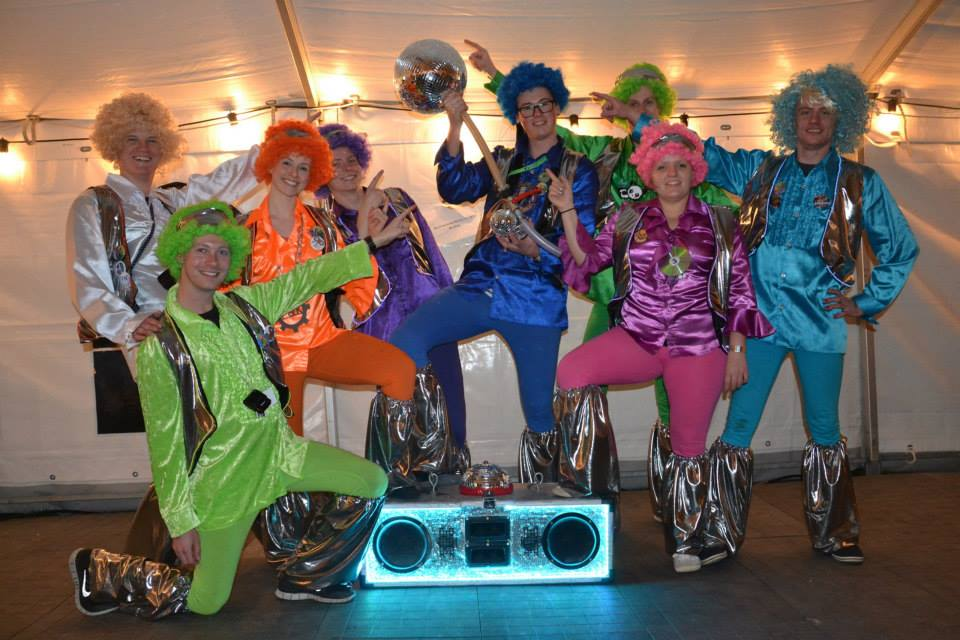
\includegraphics[width=\linewidth]{fig/Diskocenteret.jpg}
\end{figure}

\vspace{3cm}

\flushleft\large\textsf{Denne drejebog tilhører:}
\flushleft\Huge\textsf{\forfatter}

\end{titlepage}

\tableofcontents

\newpage
\Overskrift{VIGTIGE TING! (M/K)}
\section{Oversigter}
\subsection{Aktivitetsskema}
\vspace{-0.5cm}
\begin{table}[H]
\begin{tabular}{*{5}{L{2.8cm}}}\specialrule{1pt}{0pt}{2pt}
\textbf{Mandag}   & \textbf{Tirsdag}    & \textbf{Onsdag}     & \textbf{Torsdag}      & \textbf{Fredag}     \\ \specialrule{1pt}{2pt}{1pt}
                  &   8.10 Rejsning!    & 8.10 Rejsning!      & 9.30 Rejsning!        & 6.10 Rejsning!      \\ %\specialrule{.25pt}{1pt}{1pt}
\Hb{10.00 Brunch} & \Hb{8.45 Morgenmad} & \Hb{8.45 Morgenmad} & \Hb{10.05 Morgenmad}  & \Hb{6.45 Morgenmad} \\ %\specialrule{.25pt}{1pt}{1pt}
13.00 Afgang fra DTU\newline14.00 Velkomst & 10.00 Krigsløb & 10.00 DTU-løb & 11.00 Forberedelse \newline 12.05 B14 & 7.20 Oprydning \newline 9.45 Afgang \\ %\specialrule{.25pt}{1pt}{1pt}
\Hb{14.30 Snacks} & \Hb{12.30 Frokost}  & \Hb{13.00 Frokost}  & \Hb{12.55 Frokost}    & \Hb{11.00 Madauktion} \\ %\specialrule{.25pt}{1pt}{1pt}
15.00 Maling af flag & 14.00 Ingeniøropgave \newline 15.15 Rektor og dekanen & 14.55 IDA & Fistforberedelse & Origofist \\ %\specialrule{.25pt}{1pt}{1pt}
\Hb{17.30 Aftensmad} & \Hb{18.00 Aftensmad} & \Hb{18.30 Aftensmad} & \Hb{18.15 Aftensmad} & \Hb{12.00 Pizza} \\ %\specialrule{.25pt}{1pt}{1pt}
20.00 Natløb & 20.00 Mande/dameaften & 19.30 FN Topmøde & 21.00 FISTING & ??.?? Kælderbar \\ \specialrule{1pt}{1pt}{0pt}
\end{tabular}
\end{table}

\subsection{Tjanseskema}
\vspace{-0.5cm}
\begin{table}[H]
\begin{tabular}{l *{5}{L{2.1cm}}}
\specialrule{1pt}{0pt}{2pt}
\textbf{Tjans}  & \textbf{Mandag}       & \textbf{Tirsdag}      & \textbf{Onsdag}       & \textbf{Torsdag}      & \textbf{Fredag}       \\ \specialrule{1pt}{2pt}{1pt}
Oprydning       &                       & \cmighty{Skotland}    & \cstive{Australien}   & \chemorides{Ølympen}  & \crandildo{Brasilien} \\ \specialrule{.25pt}{1pt}{1pt}
Før morgenmad   &                       & \crandildo{Brasilien} & \cbuddha{Sydøstasien} & \ckarla{Vikingeland}  & \cclint{'Murica}      \\ \specialrule{.25pt}{1pt}{1pt}
Efter morgenmad &                       & \cclint{'Murica}      & \cfarav{Egypten}      & \cstive{Australien}   & \cbuddha{Sydøstasien} \\ \specialrule{.25pt}{1pt}{1pt}
Før frokost     &                       & \cstive{Australien}   & \crandildo{Brasilien} & \cmighty{Skotland}    &                       \\ \specialrule{.25pt}{1pt}{1pt}
Efter frokost   &                       & \chemorides{Ølympen}  & \ckarla{Vikingeland}  & \cfarav{Egypten}      &                       \\ \specialrule{.25pt}{1pt}{1pt}
Før aftensmad   & \cbuddha{Sydøstasien} & \cfarav{Egypten}      & \chemorides{Ølympen}  & \Hashtag{FIST}        &                       \\ \specialrule{.25pt}{1pt}{1pt}
Efter aftensmad & \cclint{'Murica}      & \ckarla{Vikingeland}  & \cmighty{Skotland}    & \Hashtag{FIST}        &                       \\ \specialrule{1pt}{1pt}{0pt}
\end{tabular}
\end{table}

\subsection{Ædruvagter}
\vspace{-0.5cm}
\begin{table}[H]
\centering
\begin{tabu}{l *{4}{L{2.8cm}}}                                          \specialrule{1pt}{0pt}{2pt}
\rowfont{\bfseries} & Mandag 13.00 Tirsdag 18.00    & Tirsdag 18.00 Onsdag 18.00   & Onsdag 18.00 Torsdag 18.00   & Torsdag 18.00 Fredag 12.00   \\ \specialrule{1pt}{2pt}{2pt}
Dagsansvarlig       & \farav    & \buddha   & \randildo & \mighty    \\ \specialrule{0pt}{1pt}{1pt}
Kørselsansvarlig    & \karla    & \stive    & \clint    & \hemorides \\ \specialrule{1pt}{2pt}{0pt}
\end{tabu}
\end{table}
\clearpage
\section{Russerne}

\subsection{Retningshold}

\vspace{-0.6cm}
\begin{figure}[H]
\centering
\subfloat{
\begin{tabular}{L{7cm}}\specialrule{1pt}{0pt}{2pt}
\textbf{BioTek - \Stive}            \\ \specialrule{1pt}{2pt}{1pt}
Annemette XXXXX                  \\ \specialrule{.25pt}{1pt}{1pt}
Jeppe Sode XXXX                     \\ \specialrule{.25pt}{1pt}{1pt}
Karen Marie	XXXXXX               \\ \specialrule{.25pt}{1pt}{1pt}
Katja K XXX                      \\ \specialrule{.25pt}{1pt}{1pt}
Lars Christian XXXXXX     \\ \specialrule{.25pt}{1pt}{1pt}
Vanessa XXXXXX                \\ \specialrule{.25pt}{1pt}{1pt}
Tanya Inger XXXXXX         \\ \specialrule{.25pt}{1pt}{1pt}
                                    \\ \specialrule{1pt}{1pt}{0pt}
\end{tabular}}
\hfill
\subfloat{
\begin{tabular}{L{7cm}}\specialrule{1pt}{0pt}{2pt}
\textbf{Elektro\Hashtag{Tosse} - \Mighty}  \\ \specialrule{1pt}{2pt}{1pt}
Johnny Martin XXXXXXXX     \\ \specialrule{.25pt}{1pt}{1pt}
Nick Hashan XXXXX       \\ \specialrule{.25pt}{1pt}{1pt}
Peter Iwer XXXXX         \\ \specialrule{.25pt}{1pt}{1pt}
Sajeel XXXXXX                     \\ \specialrule{.25pt}{1pt}{1pt}
Sebastian XXXXX              \\ \specialrule{.25pt}{1pt}{1pt}
Markus XXXXXXX           \\ \specialrule{.25pt}{1pt}{1pt}
Christian Berg XXXXX             \\ \specialrule{.25pt}{1pt}{1pt}
Kristian XXXXXX                   \\ \specialrule{1pt}{1pt}{0pt}
\end{tabular}}
\end{figure}
\vspace{-0.8cm}

\begin{figure}[H]
\centering
\subfloat{
\begin{tabular}{L{7cm}}\specialrule{1pt}{0pt}{2pt}
\textbf{Kemi - \Randildo}           \\ \specialrule{1pt}{2pt}{1pt}
Josefine XXXXXXXXX       \\ \specialrule{.25pt}{1pt}{1pt}
Malina XXXXX             \\ \specialrule{.25pt}{1pt}{1pt}
Morten XXXX                       \\ \specialrule{.25pt}{1pt}{1pt}
Oktay XXXX                          \\ \specialrule{.25pt}{1pt}{1pt}
Rasmus Lykke XXXX              \\ \specialrule{.25pt}{1pt}{1pt}
Thorbjørn XXXX            \\ \specialrule{.25pt}{1pt}{1pt}
William XXXX                    \\ \specialrule{1pt}{1pt}{0pt}
\end{tabular}}
\hfill
\subfloat{
\begin{tabular}{L{7cm}}\specialrule{1pt}{0pt}{2pt}
\textbf{P\&K - \Karla}  \\ \specialrule{1pt}{2pt}{1pt}
Christian XXXXX                 \\ \specialrule{.25pt}{1pt}{1pt}
Gisli Tomas XXXXX              \\ \specialrule{.25pt}{1pt}{1pt}
Ingvi XXXXXX                    \\ \specialrule{.25pt}{1pt}{1pt}
Joachim Holm XXXX                \\ \specialrule{.25pt}{1pt}{1pt}
Nicklas XXXX                     \\ \specialrule{.25pt}{1pt}{1pt}
Søren XXXX                     \\ \specialrule{.25pt}{1pt}{1pt}
Bjarke XXXXXXXX          \\ \specialrule{1pt}{1pt}{0pt}
\end{tabular}}
\end{figure}
\vspace{-0.8cm}

\begin{figure}[H]
\centering
\subfloat{
\begin{tabular}{L{7cm}}\specialrule{1pt}{0pt}{2pt}
\textbf{MatTek - \Hemorides}        \\ \specialrule{1pt}{2pt}{1pt}
Anders XXXX XXX           \\ \specialrule{.25pt}{1pt}{1pt}
Emil Nørgaard XXXX                 \\ \specialrule{.25pt}{1pt}{1pt}
Josephine Byskov XXXX             \\ \specialrule{.25pt}{1pt}{1pt}
Morten XXXXX               \\ \specialrule{.25pt}{1pt}{1pt}
Morten Ryberg XXXX             \\ \specialrule{.25pt}{1pt}{1pt}
Sophie Natasha XXXXXX  \\ \specialrule{.25pt}{1pt}{1pt}
Sebastian Alvan XX         \\ \specialrule{1pt}{1pt}{0pt}
\end{tabular}}
\hfill
\subfloat{
\begin{tabular}{L{7cm}}\specialrule{1pt}{0pt}{2pt}
\textbf{VBMil - \Buddha}            \\ \specialrule{1pt}{2pt}{1pt}
Anita XXXX                      \\ \specialrule{.25pt}{1pt}{1pt}
Camilla Christiane XXXX         \\ \specialrule{.25pt}{1pt}{1pt}
Magnus XXXX                          \\ \specialrule{.25pt}{1pt}{1pt}
Mette XXXX Møller              \\ \specialrule{.25pt}{1pt}{1pt}
Morten Højen XXXX            \\ \specialrule{.25pt}{1pt}{1pt}
Nikola XXXXX                    \\ \specialrule{.25pt}{1pt}{1pt}
                    \\ \specialrule{1pt}{1pt}{0pt}
\end{tabular}}
\end{figure}
\vspace{-0.8cm}

\begin{figure}[H]
\centering
\subfloat{
\begin{tabular}{L{7cm}}\specialrule{1pt}{0pt}{2pt}
\textbf{Byg - \Clint}               \\ \specialrule{1pt}{2pt}{1pt}
Frederik XXXX                      \\ \specialrule{.25pt}{1pt}{1pt}
Lasse XXX                        \\ \specialrule{.25pt}{1pt}{1pt}
Maria Rotne XXX                \\ \specialrule{.25pt}{1pt}{1pt}
Markus Pai XXXXX                 \\ \specialrule{.25pt}{1pt}{1pt}
Natasja Emilie XX            \\ \specialrule{.25pt}{1pt}{1pt}
Alexander XXXXXX           \\ \specialrule{.25pt}{1pt}{1pt}
Rikke XXXXX                      \\ \specialrule{1pt}{1pt}{0pt}
\end{tabular}}
\hfill
\subfloat{
\begin{tabular}{L{7cm}}\specialrule{1pt}{0pt}{2pt}
\textbf{FysNan - \Farav}            \\ \specialrule{1pt}{2pt}{1pt}
\Hashtag{SørgeligtFremmøde}         \\ \specialrule{.25pt}{1pt}{1pt}
\Hashtag{DeKunneIkkeDenDag}         \\ \specialrule{.25pt}{1pt}{1pt}
\Hashtag{DeSkulleAlleSammenTilDart} \\ \specialrule{.25pt}{1pt}{1pt}
\Hashtag{HvorErKABS'Russer?}        \\ \specialrule{.25pt}{1pt}{1pt}
\Hashtag{DetErNokBedstForAlle}       \\ \specialrule{.25pt}{1pt}{1pt}
                                    \\ \specialrule{.25pt}{1pt}{1pt}
                                    \\ \specialrule{1pt}{1pt}{0pt}
\end{tabular}}
\end{figure}

\subsection{Tværhold}

\vspace{-0.6cm}
\begin{figure}[H]
\centering
\subfloat{
\begin{tabular}{L{7cm}}\specialrule{1pt}{0pt}{2pt}
\textbf{\cfarav{Egypten - Farav Ikmer}}     \\ \specialrule{1pt}{2pt}{1pt}
Morten XXX XX (MatTek)              \\ \specialrule{.25pt}{1pt}{1pt}
Sajeel XXX (Elektro)                    \\ \specialrule{.25pt}{1pt}{1pt}
Annemette XXX (BioTek)                 \\ \specialrule{.25pt}{1pt}{1pt}
Anita XXXXX (Miljø)                      \\ \specialrule{.25pt}{1pt}{1pt}
Søren XXXXX (P\&K)                       \\ \specialrule{.25pt}{1pt}{1pt}
William XXXX (Kemi)                     \\ \specialrule{.25pt}{1pt}{1pt}
                                            \\ \specialrule{1pt}{1pt}{0pt}
\end{tabular}}
\hfill
\subfloat{
\begin{tabular}{L{7cm}}\specialrule{1pt}{0pt}{2pt}
\textbf{\ckarla{Vikingeland - Karla K. Kløvehjerte}}\\ \specialrule{1pt}{2pt}{1pt}
Lasse XXXX (Byg)                          \\ \specialrule{.25pt}{1pt}{1pt}
Magnus XXX (Miljø)                          \\ \specialrule{.25pt}{1pt}{1pt}
Alexander XXXX (Byg)             \\ \specialrule{.25pt}{1pt}{1pt}
Sophie Natasha XXXXX (MatTek)        \\ \specialrule{.25pt}{1pt}{1pt}
Vanessa XXXXX (BioTek)               \\ \specialrule{.25pt}{1pt}{1pt}
Morten XXXX (Kemi)                        \\ \specialrule{.25pt}{1pt}{1pt}
                                            \\ \specialrule{1pt}{1pt}{0pt}
\end{tabular}}
\end{figure}
\vspace{-0.8cm}

\begin{figure}[H]
\centering
\subfloat{
\begin{tabular}{L{7cm}}\specialrule{1pt}{0pt}{2pt}
\textbf{\crandildo{Brasilien - Randildo Bailando}}\\ \specialrule{1pt}{2pt}{1pt}
Jeppe Sode XX (BioTek)                    \\ \specialrule{.25pt}{1pt}{1pt}
Nicklas XXXX (P\&K)                      \\ \specialrule{.25pt}{1pt}{1pt}
Morten XXX XX (MatTek)           \\ \specialrule{.25pt}{1pt}{1pt}
Mette Torsberg XXXX (Miljø)               \\ \specialrule{.25pt}{1pt}{1pt}
Peter Iwer XXX XXXX (Elektro)       \\ \specialrule{.25pt}{1pt}{1pt}
Natasja Emilie XXXX (Byg)              \\ \specialrule{.25pt}{1pt}{1pt}
                                            \\ \specialrule{1pt}{1pt}{0pt}
\end{tabular}}
\hfill
\subfloat{
\begin{tabular}{L{7cm}}\specialrule{1pt}{0pt}{2pt}
\textbf{\cclint{'Murica - Clint Hardwood}}  \\ \specialrule{1pt}{2pt}{1pt}
Christian Berg XXXX (Elektro)           \\ \specialrule{.25pt}{1pt}{1pt}
Joachim Holm XXXXX (P\&K)                 \\ \specialrule{.25pt}{1pt}{1pt}
Josephine Byskov XXX (MatTek)            \\ \specialrule{.25pt}{1pt}{1pt}
Karen Marie XXXXX (BioTek)              \\ \specialrule{.25pt}{1pt}{1pt}
Morten Højen XXXX (Miljø)            \\ \specialrule{.25pt}{1pt}{1pt}
Rasmus Lykke XXXXX (Kemi)               \\ \specialrule{.25pt}{1pt}{1pt}
                                            \\ \specialrule{1pt}{1pt}{0pt}
\end{tabular}}
\end{figure}
\vspace{-0.8cm}

\begin{figure}[H]
\centering
\subfloat{
\begin{tabular}{L{7cm}}\specialrule{1pt}{0pt}{2pt}
\textbf{\cstive{Australien - Stive Irwin}}  \\ \specialrule{1pt}{2pt}{1pt}
Camilla Christiane XXXX (Miljø)         \\ \specialrule{.25pt}{1pt}{1pt}
Frederik XXXX (Byg)                        \\ \specialrule{.25pt}{1pt}{1pt}
Johnny Martin XXXXX (Elektro)   \\ \specialrule{.25pt}{1pt}{1pt}
Oktay XXX (Kemi)                           \\ \specialrule{.25pt}{1pt}{1pt}
Anders Dalsgård XXXXX (MatTek)           \\ \specialrule{.25pt}{1pt}{1pt}
Bjarke Dalhoff XXX (P\&K)           \\ \specialrule{.25pt}{1pt}{1pt}
                                            \\ \specialrule{1pt}{1pt}{0pt}
\end{tabular}}
\hfill
\subfloat{
\begin{tabular}{L{7cm}}\specialrule{1pt}{0pt}{2pt}
\textbf{\cmighty{Skotland - Mighty O'Long-John}}\\ \specialrule{1pt}{2pt}{1pt}
Christian XXXX (P\&K)                  \\ \specialrule{.25pt}{1pt}{1pt}
Emil Nørgaard XXXX (MatTek)                \\ \specialrule{.25pt}{1pt}{1pt}
Lars Chr. Vindfelt XXXX (BioTek)          \\ \specialrule{.25pt}{1pt}{1pt}
Malina Benedicte XXXX (Kemi)              \\ \specialrule{.25pt}{1pt}{1pt}
Maria  XXX Bessman (Byg)                  \\ \specialrule{.25pt}{1pt}{1pt}
Nikola XXXX (Vand)                     \\ \specialrule{.25pt}{1pt}{1pt}
                                            \\ \specialrule{1pt}{1pt}{0pt}
\end{tabular}}
\end{figure}
\vspace{-0.8cm}

\begin{figure}[H]
\centering
\subfloat{
\begin{tabular}{L{7cm}}\specialrule{1pt}{0pt}{2pt}
\textbf{\chemorides{Ølympen - Hæmorides af Ølympen}}\\ \specialrule{1pt}{2pt}{1pt}
Thorbjørn Anker Sørensen(Kemi)              \\ \specialrule{.25pt}{1pt}{1pt}
Rikke Andersen (Byg)                        \\ \specialrule{.25pt}{1pt}{1pt}
Nick Hashan Thanthrige (Elektro)            \\ \specialrule{.25pt}{1pt}{1pt}
Tanya Teglbjærg (BioTek)                    \\ \specialrule{.25pt}{1pt}{1pt}
Gisli Tomas Gudjonsson (P\&K)               \\ \specialrule{.25pt}{1pt}{1pt}
Markus Mogensen Henriksen (Elektro)         \\ \specialrule{.25pt}{1pt}{1pt}
     \\ \specialrule{1pt}{1pt}{0pt}
\end{tabular}}
\hfill
\subfloat{
\begin{tabular}{L{7cm}}\specialrule{1pt}{0pt}{2pt}
\textbf{\cbuddha{Sydøstasien - Buddha Karma Sutma}}\\ \specialrule{1pt}{2pt}{1pt}
Josefine Hvarregård XXX (Kemi)         \\ \specialrule{.25pt}{1pt}{1pt}
Ingvi XXXXXX (P\&K)                     \\ \specialrule{.25pt}{1pt}{1pt}
Sebastian XXXXX (Elektro)         \\ \specialrule{.25pt}{1pt}{1pt}
Katja XXXXX (BioTek)                     \\ \specialrule{.25pt}{1pt}{1pt}
Markus Pai XXXXX (Byg)                   \\ \specialrule{.25pt}{1pt}{1pt}
Kristian XXXX (Elektro)                 \\ \specialrule{.25pt}{1pt}{1pt}
Sebastian XXXXX (MatTek)        \\ \specialrule{1pt}{1pt}{0pt}
\end{tabular}}
\end{figure}

$$$$ % snyd og bedrag så "Kontaktinformationer" korrekt hopper ned på næste side

\subsection{Kontaktinformationer}

\begin{table}[H]
\centering
\small
\begin{tabu}{l l r l l}
\specialrule{1pt}{0pt}{2pt}
\rowfont{\bfseries}
$\boxtimes$ & Navn & Mobil & Kontakt & Nummer \\
\specialrule{1pt}{2pt}{2pt}
% Byttet væk:
%  Cecilie 'Elektro Spasser' -> Klinteborg
%  Andreas XXXX (Byg) -> Høve Strand
%  Daniel XXXX Høgh (ElTekn) -> Klinteborg
%  Christian XXX (P&K) -> Østersøen
%  Jeppe XXX-Pedersen (P\&K) -> Klintehytten

$\square$ & Alexander Neergård XXX (Byg)              & 236 3XXXX & -                    & - \\
$\square$ & Anders Dalsgaard XXX (MatTek)           & 6179 XXXX & -                     & 6179 XXXX  \\
$\square$ & Anita XXX (Miljø)                       & 2844 XXXX &  Bent XXX        & 5099 XXXX  \\
$\square$ & Annemette XXX (BioTek)                  & 6065 XXXX & -                     & -         \\
$\square$ & Bjarke Dalhoff XXX (P\&K)            & 3028 XXXX & Hanne XXX     & 2819 XXXX  \\
$\square$ & Camilla Christiane XXX (Miljø)          & 2512 XXXX & Ilse XXX          & 3027 XXXX  \\
$\square$ & Christian Berg XXX (ElTekn)             & 4076 XXXX & ?                     & ?         \\
$\square$ & Christian XXX (P\&K)                   & 2125 XXXX & -                     & -         \\
$\square$ & Emil Nørgaard XXX (MatTek)                 & 3064 XXXX & Vibeke XXX          & 6224 XXXX  \\
$\square$ & Frederik XXX (Byg)                          & 2829 XXXX & Kenneth XXX         & 5060 XXXX  \\
$\square$ & Ingvi XXX (P\&K)                      & 3172 XXXX & -                     & -         \\
$\square$ & Gisli Tomas XXX (P\&K) \textbf{Island}& +35 4821 XXXX & -                 & -         \\
$\square$ & Jeppe Sode XXX (BioTek)                     & 2421 XXXX & -                     & -         \\
$\square$ & Joachim Holm XXX (P\&K)                  & 2390 XXXX & Ulla XXX             & 2815 XXXX  \\
$\square$ & Johnny Martin XXX XXX (ElTekn)     & 6074 XXXX & -                     & -         \\
$\square$ & Josefine XXX XXX (Kemi)         & 2171 XXXX & William XX & 2611 XXXX  \\
$\square$ & Josephine XX XX (MatTek)             & 9392 XXXX & Lene XXX           & 2488 XXXX  \\
$\square$ & Karen Marie XXX (BioTek)               & 2081 XXXX & Berte XXX        & 4588 XXXX  \\
$\square$ & Kristian XXX (ElTekn)                   & 2062 XXXX & Krista XXX       & 2530 XXXX  \\
$\square$ & Katja XXX (BioTek)                      & 2990 XXXX & Mor                   & 3025 XXXX  \\
$\square$ & Lars Christian XXX XXX (BioTek)     & 2857 XXXX & Otilia XXX (engelsk) & 5034 XXXX  \\
$\square$ & Lasse XXX (Byg)                           & 2857 XXXX & -                     & -         \\
$\square$ & Magnus XXX (Miljø)                           & -         & -                     & -         \\
$\square$ & Malina  XXX (Kemi) \textbf{senere}        & 5356 XXXX & Michael XXX        & 2890 XXXX  \\
$\square$ & Maria Rotne XXX (Byg)                   & 3084 XXXX & Annette XXX      & 3084 XXXX  \\
$\square$ & Markus Mogensen XXX (ElTekn)           & 2782 XXXX & Jes XXX         & 4044 XXXX  \\
$\square$ & Markus Pai XXX (Byg)                    & 2855 XXXX & Hans XXX         & 2129 XXXX  \\
$\square$ & Mette XXX (Miljø)               & 4126 XXXX & Søren XXX          & 4242 XXXX  \\
$\square$ & Morten XXX XXX (MatTek)               & 2980 XXXX & -                     & -         \\
$\square$ & Morten XXX (Kemi)                         & -         & Far                   & 3079 XXXX  \\
$\square$ & Morten Højen XXX (Miljø)             & 2330 XXXX & Britta XXX Højen & 3031 XXXX  \\
$\square$ & Morten Ryberg XXX (MatTek)             & 5190 XXXX & Susanne XXX     & 5190 XXXX  \\
$\square$ & Natasja Emilie XXX (Byg)               & 2369 XXXX & Karina XXX (Mor)   & 2921 XXXX  \\
$\square$ & Nick Hashan XXX XXX (ElTekn)       & 5239 XXXX & -                     & -         \\
$\square$ & Nicklas XXX (P\&K)                       & 2989 XXXX & Gitte XXX         & 2710 XXXX  \\
$\square$ & Nikola XXX (Miljø)                     & 5244 XXXX & -                     & -         \\
$\square$ & Oktay XXX (Kemi)                            & 3172 XXXX & Veli XXX             & 3123 XXXX  \\
$\square$ & Peter Iwer XXX XX (ElTekn)         & 6048 XXXX & -                     & -         \\
$\square$ & Rasmus Lykke XXX (Kemi)                & 4018 XXXX & -                     & -         \\
$\square$ & Rikke XXX (Byg)                         & 3028 XXXX & Line XXX         & 2894 XXXX  \\
$\square$ & Sajeel XXX (ElTekn)                      & 5353 XXXX & Mor                   & 2991 XXXX  \\
$\square$ & Sebastian XXX (ElTekn)               & 2328 XXXX & Mor                   & 2665 XXXX  \\
$\square$ & Sebastian Alvan XXX (MatTek)          & 6165 XXXX & -                     & - \\
$\square$ & Sophie XXX XX (MatTek)        & 2287 XXXX & -                     & -         \\
$\square$ & Søren XXX (P\&K)                       & 7120 XXXX & Lene XXX        & 6162 XXXX  \\
$\square$ & Tanya Inger XXX (BioTek)         & 2853 XXXX & Andreas XXX    & 2086 XXXX  \\
$\square$ & Thorbjørn Anker XXX (Kemi)              & 2045 XXXX & Jesper XXX       & 4140 XXXX  \\
$\square$ & Vanessa XXX (BioTek)                & 2862 XXXX & Lene XXX     & 2862 XXXX  \\
$\square$ & William XXX (Kemi)                      & 4111 XXXX & Helle XXX          & 2948 XXXX  \\

\end{tabu}
\end{table}
\clearpage
\section{Tidsplan}
\subsection{Søndag}
\begin{longtable}{L{1cm} L{4.5cm} L{5.5cm} L{3.3cm}}\specialrule{1pt}{0pt}{2pt}
\textbf{Tid} & \textbf{Aktivitet}       & \textbf{Bemærkning/sted/materialer}            & \textbf{Ansvarlige}   \\ \specialrule{.25pt}{1pt}{1pt}
09.00        & Varevogn hentes          & Europcar:  Firskovvej 8, 2800 Kgs. Lyngby      & \Hyttebums{Elizabeth} \\ \specialrule{.25pt}{1pt}{1pt}
09.15        & Anlæg og fustager hentes & Adresse: Dalen 19, 2860 Søborg                 & \Hyttebums{Elizabeth} \\ \specialrule{.25pt}{1pt}{1pt}
??           & Varer hentes i ??        & Adresse: ??                                    & \Hyttebums{Elizabeth} \\ \specialrule{.25pt}{1pt}{1pt}
12.00        & Varevogn køres tilbage til DTU, og badekar m.m. læsses ind. & Husk fustage fra B14! Ligger foran deres kontor fra kl. 12                                                     & \Hyttebums{Elizabeth}, \farav                                          \\ \specialrule{.25pt}{1pt}{1pt}
?            & ?                        & ?                                              & ?                     \\ \specialrule{1pt}{1pt}{0pt}
\end{longtable}

\subsection{Mandag}
\begin{longtable}{L{1cm} L{4.5cm} L{5.5cm} L{3.3cm}}\specialrule{1pt}{0pt}{2pt}
\textbf{Tid} & \textbf{Aktivitet} & \textbf{Bemærkning/sted/materialer} & \textbf{Ansvarlige}\\ \specialrule{1pt}{2pt}{1pt}

08.00 & Afgang fra DTU! & Metro: ??? & \Hyttebums{Elizabeth, Jack} og \farav \\ \specialrule{.25pt}{1pt}{1pt}
09.00 & Offentlig transport hæhæhæ & Endestation: ??? & \Hyttebums{William} \\ \specialrule{.25pt}{1pt}{1pt}
?? & \Hyttebums{William Turn-on} hentes & Adresse: ??? & \farav \\ \specialrule{.25pt}{1pt}{1pt}
10.00 & Hytten klargøres & Se to do liste & \farav og \Hyttebums{Hyttebumser} \\ \specialrule{.25pt}{1pt}{1pt}
10.00 & Vektorer mødes hos \karla til brunch & Kampsax 2411 & Alle vektorer \\ \specialrule{.25pt}{1pt}{1pt}
11.00 & Øllene ankommer & Gården \Hashtag{HuskDinVærdighed} & \farav \\ \specialrule{.25pt}{1pt}{1pt}
12.00 & Afgang fra Kampsax, indkøb af øl + sodavand til busturen & Husk streglister til bussen & Alle vektorer \\ \specialrule{.25pt}{1pt}{1pt}
12.15 & Klar til at modtage russer! & \hemorides har kontakt til bus. Lars (\mighty) har fødselsdag! & Alle vektorer \\ \specialrule{.25pt}{1pt}{1pt}
13.00 & Afgang mod Center Sjælland! & \karla ringer til \farav & Alle vektorer \\\specialrule{.25pt}{1pt}{1pt}
13.45 & \karla ringer til \farav og fortæller hvor langt de er & Broskååååååål! & \karla \\\specialrule{.25pt}{1pt}{1pt}
14.00  & Ankomst til Center Sjælland & Alle venter på gårdspladsen & \hemorides og \farav  \\\specialrule{.25pt}{1pt}{1pt}
14.05 & Velkomsttale + regler & På gårdspladsen & \farav \\\specialrule{.25pt}{1pt}{1pt}
14.30 & Hygge i tværhold udenfor + snacks fra køkkenet & Alle giver en kasse til sit hold - husk at spørge om nogen vil have sodavand \Hashtag{Liking} & Alle vektorer + \Hyttebums{hyttebumser} \\\specialrule{.25pt}{1pt}{1pt}
15.00 & Maling af flag og hygge, udlevering af missionskort & Rundt omkring udenfor - hvis indenfor husk sorte sække under & \farav + \karla \\\specialrule{.25pt}{1pt}{0pt}
\end{longtable}

\clearpage
\section*{Side 9}

\begin{figure}[H]
\centering

\includegraphics[width=13cm]{fig/Side9.png}
\end{figure}
\Hashtag{ErDinSide9pigeOgsåEnMand?}

\clearpage
\section*{Side 9\sfrac{3}{4}}
\Hashtag{BassOpIKussenMasserMasserBassIKussen}
\begin{figure}[H]
\centering

\includegraphics[width=13cm]{fig/Skoegen.jpg}
\end{figure}

\clearpage
\subsection*{Mandag fortsat}
\begin{longtable}{L{1cm} L{4.5cm} L{5.5cm} L{3.3cm}}\specialrule{1pt}{0pt}{2pt}
\textbf{Tid} & \textbf{Aktivitet} & \textbf{Bemærkning/sted/materialer} & \textbf{Ansvarlige}\\ \specialrule{1pt}{2pt}{1pt}
15.15 & Uddeling af nabobreve & Ved siden af Center Sjælland & \karla \\\specialrule{.25pt}{1pt}{1pt}
17.15 & Sydøstasien sendes ud til køkkenet & De skal vente \textbf{uden for} køkkenet! & \buddha \\\specialrule{.25pt}{1pt}{1pt}
17.30 & Alle sendes i spisesalen & HUSK AT VASKE HÆNDER!!! Lars (\mighty) har fødselsdag! &  \Hyttebums{Hyttebumser} og \farav + \karla \\\specialrule{.25pt}{1pt}{1pt}
19.00 & Aftensmad slut & 'Murica rydder op, fortæl om sladderkassen, tjanse/aktivitetsskema, RISK kort og at der kommer natløb & \farav + \karla \\\specialrule{.25pt}{1pt}{1pt}
19.05 & Hurtigt kaosmøde & Vektorværelset \Hashtag{HverdagsSM} & Alle vektorer og KABS \\\specialrule{.25pt}{1pt}{1pt}
19.30 & Opsætning af natløb & Husk trylledej & Alle vektorer \\\specialrule{.25pt}{1pt}{1pt}
19.50 & Præsentation af natløb & Samling i spisesalen, BESTIKKELSE!!! & \clint og \karla \\\specialrule{.25pt}{1pt}{1pt}
20.00 & Natløb & \karla tager billeder & \clint og \karla \\\specialrule{.25pt}{1pt}{1pt}
22.00 & Natløb slut & Fri leg + oprydning, husk trylledej & Alle voksne  \\\specialrule{.25pt}{1pt}{1pt}
00.00 & NATMAAAAAD! & Spisesalen & \Hyttebums{Piraterne} \\\specialrule{.25pt}{1pt}{1pt}
02.00 & DRUKSTOOOOP! & Ha gaaaaay! & \buddha og \stive \\\specialrule{.25pt}{1pt}{1pt}
\textbf{FIST} & \textbf{FIST} & \textbf{FIST} & \textbf{FIST} \\\specialrule{1pt}{1pt}{0pt}

\end{longtable}


\subsection{Tirsdag}
\begin{longtable}{L{1cm} L{4.5cm} L{5.5cm} L{3.3cm}}\specialrule{1pt}{0pt}{2pt}
\textbf{Tid} & \textbf{Aktivitet} & \textbf{Bemærkning/sted/materialer} & \textbf{Ansvarlige}\\ \specialrule{1pt}{2pt}{1pt}

02.00 & DRUKSTOOOOP! & Ha gaaaaay! & \buddha og \stive \\\specialrule{.25pt}{1pt}{1pt}
07.15 & Ølansvarlige vågner og gør status på øl & 100 bajere & \mighty + \buddha \\\specialrule{.25pt}{1pt}{1pt}
07.30 & Vektorer vækkes & I dag er der morgenfest! & \farav + \karla \\\specialrule{.25pt}{1pt}{1pt}
07.35 & Skotland og Brasilien sendes til tjanser & Oprydning rundt omkring og køkkenet & \mighty og \randildo \\\specialrule{.25pt}{1pt}{1pt}
07.45 & Kaosmøde & Hent en fra køkkenet til fællesfist! & \farav + alle \\\specialrule{.25pt}{1pt}{1pt}
08.00 & Russerne vækkes & \buddha sætter Beautiful Morning på repeat & Alle voksne \\\specialrule{.25pt}{1pt}{1pt}
08.10 & Morgenrejsning & Udenfor køkkenet - husk at give beskeder & \farav, \randildo og \Hyttebums{Turn-on} \\\specialrule{.25pt}{1pt}{1pt}
08.40 & Morgenrejsning slutter-VASK HÆNDER!!! & FÅ DEM TIL AT VASKE DE FUCKING HÆNDER! & Alle voksne \\\specialrule{.25pt}{1pt}{1pt}
08.45 & Morgenmad & Spisesalen, udlever nye missionskort &  \Hyttebums{Hyttebumser} og \farav + \karla \\\specialrule{.25pt}{1pt}{1pt}
09.30 & Morgenmad slut & 'Murica rydder op, husk at fortælle at der er samling om lidt, spørg om nogen har klaret missionskort og sæt dem på kortet & \farav + \karla \\\specialrule{.25pt}{1pt}{1pt}
09.35 & Klargøring af krigsløb & Alle steder \Hashtag{DinMor} & Alle! \\\specialrule{.25pt}{1pt}{1pt}
09.50 & Samling og introduktion af krigsløb	&	Spisesalen	& \randildo \\\specialrule{.25pt}{1pt}{1pt}
10.00 & Krigsløb! & Alle steder & \randildo \\\specialrule{.25pt}{1pt}{1pt}
12.00 & Krigsløb slutter - oprydning & Australien sendes i køkkenet & \stive + alle vektorer \\\specialrule{.25pt}{1pt}{1pt}
12.05 & Klargøring til ingeniøropgaven & Materialer lægges klar til holdene & \buddha og \hemorides \\\specialrule{.25pt}{1pt}{1pt}
12.20 & Alle sendes i spisesalen & Rene hænder gi'r raske venner! & \farav + \karla \\\specialrule{.25pt}{1pt}{1pt}
12.30 & Frokost + Fortæl om ædrudag & Spisesalen &  \Hyttebums{Hyttebumser} og \farav + \karla \\\specialrule{.25pt}{1pt}{1pt}
13.30 & Frokost slut! & Ølympen rydder op. Husk at sige at vi mødes igen til ingeniøropgaven & \farav \karla \hemorides \\\specialrule{.25pt}{1pt}{1pt}
14.00 & Ingeniøropgaven præsenteres & Rundt omkring & \buddha og \hemorides \\\specialrule{.25pt}{1pt}{1pt}
14.30 & Der gøres klar til rektor og dekanen & Spisesalen (eller udenfor?) - stole/borde opsættes & \farav, \mighty, \clint og \stive \\\specialrule{.25pt}{1pt}{1pt}
15.10 & Samling i spisesalen & Spisesalen & \farav + \karla \\\specialrule{.25pt}{1pt}{1pt}
15.15 & Rektor og dekanen ankommer & Spisesalen & \farav + \karla \\\specialrule{.25pt}{1pt}{1pt}
15.55 & Rektor og dekanen tager afsted igen - MADNESS CONTINUES! & Gør klar til præsentation af krigsvåben & \farav + \karla \\\specialrule{.25pt}{1pt}{1pt}
16.00 & Præsentation af krigsvåben & Rundt omkring & \buddha og \hemorides \\\specialrule{.25pt}{1pt}{1pt}
16.15 & Vektorerne + KABS voterer om hvem der vinder & Vinderen kåres og modtager arméere & \buddha og \hemorides \\\specialrule{.25pt}{1pt}{1pt}
16.30 & Fri leg + casual ølspilsteori & Alle steder! & ALLE! \\\specialrule{.25pt}{1pt}{1pt}
17.30 & Egypten sendes ud til piraterne & Køkkenet & \farav \\\specialrule{.25pt}{1pt}{1pt}
17.50 & Alle sendes i køkkenet & Fuck liking, vask hænder! & \farav + \karla \\\specialrule{.25pt}{1pt}{1pt}
18.00 & Ædruvestover\textbf{DRAGE}lse!!!! (og aftensmad) & \farav + \karla overdrager vestene til \buddha og \stive, og der bundes en fucking bajer og cocio. &  \Hyttebums{Hyttebumser} og \farav + \karla \\\specialrule{.25pt}{1pt}{1pt} 
19.00 & Aftensmad slut & Vikingerne rydder op, husk info om mande/dameaften & \buddha + \stive \\\specialrule{.25pt}{1pt}{1pt}
19.20 & Kaosmøde & Vektorværelset & Alle \\\specialrule{.25pt}{1pt}{1pt}
19.30 & Forberedelse til drenge/pige aften & \Hyttebums{Porn} skal stege bacon & \buddha og \randildo \\\specialrule{.25pt}{1pt}{1pt}
19.50 & Samling inden drenge/pigeaften & Spisesalen & \buddha og \randildo \\\specialrule{.25pt}{1pt}{1pt}
20.00 & Drenge/pigeaften begynder! & Se bilagene & \buddha og \randildo \\\specialrule{.25pt}{1pt}{1pt}
22.00 & Lille prinsesse-battle & Spisesalen & \buddha og \randildo \\\specialrule{.25pt}{1pt}{1pt}
22.30 & FIST & Bag i bussen & FIST \\\specialrule{.25pt}{1pt}{1pt}
00.00 & Beskøjter & Spisesalen?! & \Hyttebums{Piraterne} \\\specialrule{.25pt}{1pt}{1pt}
02.00 & \randildo og \clint har drukket NOK! & KABS har IKKE drukket nok & \randildo og \clint \\\specialrule{1pt}{1pt}{0pt}

\end{longtable}


\subsection{Onsdag (ædrudag!)}

\Hashtag{KanDuHellerIkkeFåCocioNok}
\begin{longtable}{L{1cm} L{4.5cm} L{5.5cm} L{3.3cm}}\specialrule{1pt}{0pt}{2pt}
\textbf{Tid} & \textbf{Aktivitet} & \textbf{Bemærkning/sted/materialer} & \textbf{Ansvarlige}\\ \specialrule{1pt}{2pt}{1pt}

02.00 & \randildo og \clint har drukket NOK! & \Hashtag{ViFårSe} & \randildo og \clint \\\specialrule{.25pt}{1pt}{1pt}
07.15 & Ølansvarlige vågner og gør status på øl & Morgenbajs! Eller nårh nej... & \mighty + \buddha \\\specialrule{.25pt}{1pt}{1pt}
07.30 & Vektorer vækkes & \karla findes hos en rus & \buddha + \stive \\\specialrule{.25pt}{1pt}{1pt}
07.35 & Australien og Indien sendes til tjanser & Oprydning rundt omkring og køkkenet & \stive og \buddha \\\specialrule{.25pt}{1pt}{1pt}
07.45 & Kaosmøde & Hent en fra køkkenet til fællesfist! & Alle voksne og \buddha \\\specialrule{.25pt}{1pt}{1pt}
08.00 & Russerne vækkes & \buddha sætter Morgenfest på repeat& Alle voksne \\\specialrule{.25pt}{1pt}{1pt}
08.10 & Morgenrejsning & Udenfor køkkenet - husk at give beskeder \Hashtag{ædrudag!}&  \clint, \farav, \Hyttebums{Elizabeth}, \buddha og \hemorides \\\specialrule{.25pt}{1pt}{1pt}
08.40 & Rejsningen er dalet igen & Husk at vaske hænder! & Alle voksne \\\specialrule{.25pt}{1pt}{1pt}
08.45 & Morgenmad, udlevering af nye missionskort & Spisesalen & \Hyttebums{Piraterne} og \buddha + \stive \\\specialrule{.25pt}{1pt}{1pt}
09.30 & Morgenmad slut & Egypten rydder op, husk at fortælle at der er samling om lidt. Spørg om der er nogen der har klaret missioner og sæt dem på kortet & \buddha + \stive \\\specialrule{.25pt}{1pt}{1pt}
09.50 & Samling og introduktion af DTU-løb	&	Spisesalen	& \buddha \\\specialrule{.25pt}{1pt}{1pt}
10.00 & Red Bull ankommer & \Hashtag{KOFFEIIIIIIIN!} & \farav \\\specialrule{.25pt}{1pt}{1pt}
10.00 & DTU-løb & Alle steder & \buddha \\\specialrule{.25pt}{1pt}{1pt}
12.00 & DTU-løb slutter & Ryd op efter jer selv & Alle vektorer \\\specialrule{.25pt}{1pt}{1pt}
12.30 & Brasilien sendes i kabyssen &  Køkkenet & \randildo \\\specialrule{.25pt}{1pt}{1pt}
12.50 & Russerne sendes i spisesalen & Skrubbe skrubbe hænder & \buddha + \stive \\\specialrule{.25pt}{1pt}{1pt}
13.00 & SÅ' DER SERVERET! & Spisesalen & \Hyttebums{Piraterne} og \buddha + \stive \\\specialrule{.25pt}{1pt}{1pt}
14.00 & STOP MED AT SPISE! & Fortæl at der er fri hygge og at IDA kommer. Vikinger rydder op & \buddha + \stive \\\specialrule{.25pt}{1pt}{1pt}
14.05 & Hyggespil og fri leg & OVERALT! & Alle \\\specialrule{.25pt}{1pt}{1pt}
14.30 & Der gøres klar til IDAs præsentation & Spisesalen (Udenfor?) - sæt stole/borde op & \buddha, \hemorides, \randildo og \farav \\\specialrule{.25pt}{1pt}{1pt}
14.50 & Russerne samles inden IDA & Spisesalen & \buddha + \stive \\\specialrule{.25pt}{1pt}{1pt}
14.55 & IDA ankommer & Spisesalen & \buddha + \stive \\\specialrule{.25pt}{1pt}{1pt}
15.30 & IDA siger farvel og tak & Spisesalen - bliv derinde & \buddha + \stive \\\specialrule{.25pt}{1pt}{1pt}
15.35 & Introduktion af FN-konventionen & Spisesalen & \farav \\\specialrule{.25pt}{1pt}{1pt}
15.45 & Skrivning af taler i tværhold & Alle steder & Alle \\\specialrule{.25pt}{1pt}{1pt}
18.00 & Der overDRAGES! & \buddha og \stive gi'r stafetten videre til \randildo og \clint & \buddha, \stive, \randildo og \clint \\\specialrule{.25pt}{1pt}{1pt}
18.01 & Egypten sendes i køkkenet & Walk like an Egyptian! \farav gør talerstolen og FN-mærkerne klar. & \farav \\\specialrule{.25pt}{1pt}{1pt}
18.20 & Kølhaling af russer & Vask hændeeeeeer! & \randildo + \clint \\\specialrule{.25pt}{1pt}{1pt}
18.30 & Beskøjter og rom & Spisesalen & \Hyttebums{Piraterne} \randildo + \clint \\\specialrule{.25pt}{1pt}{1pt}
19.30 & Aftensmad slut - alle bliver siddende & Vikingerne rydder af bordene, men vasker ikke op endnu & \farav og \randildo + \clint  \\\specialrule{.25pt}{1pt}{1pt} 
19.30 & FN-topmøde! & Spisesalen, \Hyttebums{Piraterne} skal holde første tale! & \farav, \randildo + \clint \\\specialrule{.25pt}{1pt}{1pt}
21.00 & Topmødet er slut, FN-delegationen voterer og finder den bedste tale & Spisesalen & Alle vektorer + KABS \\\specialrule{.25pt}{1pt}{1pt}
21.05 & Vinderen kåres, herefter fri leg & Vikingerne sendes ud til opvask igen & \farav og \karla \\\specialrule{.25pt}{1pt}{1pt}
21.10 & FRI (ædru) FIST TIL DØDEN! & Hele verden & Alle \\\specialrule{.25pt}{1pt}{1pt}
00.00 & Mellemsnacking & Spisesalen & \Hyttebums{Hyttebombz} \\\specialrule{.25pt}{1pt}{1pt}
02.00 & \mighty og \hemorides stopper med at drikke & NÅRH NEJ DET GJORDE DE JO ALLIGEVEL IKKE! & \mighty og \hemorides \\\specialrule{1pt}{1pt}{0pt}

\end{longtable}


\newpage
\subsection{Torsdag \Hashtag{ErDerFuckingFest?!}}

\begin{longtable}{L{1cm} L{4.5cm} L{5.5cm} L{3.3cm}}\specialrule{1pt}{0pt}{2pt}
\textbf{Tid} & \textbf{Aktivitet} & \textbf{Bemærkning/sted/materialer} & \textbf{Ansvarlige}\\ \specialrule{1pt}{2pt}{1pt}

02.00 & \mighty og \hemorides stopper med at drikke & NÅRH NEJ DET GJORDE DE JO ALLIGEVEL IKKE! & \mighty og \hemorides \\\specialrule{.25pt}{1pt}{1pt}
08.30 & Ølansvarlige vågner og gør status på øl & VI MÅ DRIKKE IGEN! & \mighty og \buddha \\\specialrule{.25pt}{1pt}{1pt}
08.45 & Vektorer vækkes & MORGENFEST! & \randildo + \clint \\\specialrule{.25pt}{1pt}{1pt}
08.50 & Ølympen og Vikingeland vækkes og sendes til tjanser & Oprydning + køkken & \hemorides og \karla \\\specialrule{.25pt}{1pt}{1pt}
09.00 & KAOSmøde & Kidnap en \Hyttebums{Turn-On} & Alle voksne \\\specialrule{.25pt}{1pt}{1pt}
09.20 & Russerne vækkes, \hemorides sætter festaften sedler op & \buddha sætter Den Dejligste Morgen i 100 År på repeat & Alle \\\specialrule{.25pt}{1pt}{1pt}
09.30 & Morgenrejsning! & \Hashtag{HarDuSnacketEnRusIDag?} & \randildo, \buddha, \mighty og \Hyttebums{Jack og Elizabeth} \\\specialrule{.25pt}{1pt}{1pt}
10.00 & Morgenrejsning slutter - VASK HÆNDER! & Rene venner gi'r raske hænder &  Alle \\\specialrule{.25pt}{1pt}{1pt}
10.05 & Morgenmad, udlevering af nye missionskort & Rasmus (\clint) har fødselsdag! & \Hyttebums{Piraterne} og  \randildo + \clint \\\specialrule{.25pt}{1pt}{1pt}
10.45 & Morgenmad er slut \Hashtag{FerneTid} & Australien rydder op, husk at fortælle om posterne til festaftenen og at Bestyrelsen kommer og sælger billetter til Rusjoint, så de skal finde deres punge. Spørg om nogen har lavet nye missionskort og sæt dem på kortet & \randildo + \clint \\\specialrule{.25pt}{1pt}{1pt}
11.00 & Fistaftensforberedelse & Mærkelige steder, husk at minde folk om at skrive sig på listerne & Alle \\\specialrule{.25pt}{1pt}{1pt}
11.30 & Oprydningsholdet gør spisesalen (eller gården?) klar til B14. \mighty undersøger hvor Bestyrelsen kan få strøm til deres fadølsanlæg fra i gården & Spisesalen og gården & \mighty og \farav \\\specialrule{.25pt}{1pt}{1pt}
11.55 & Få russerne til at finde deres punge så de kan købe billetter til rusjoint og sæt jer sammen i tværhold inden bestyrelsen kommer & Spisesalen & Alle voksne \\\specialrule{.25pt}{1pt}{1pt}
12.05 & B14 ankommer til Center Sjælland! & Spisesalen. Sav i formanden & \randildo + \clint \\\specialrule{.25pt}{1pt}{1pt}
12.25 & B14 giver gratis fadøl og sælger billetter til rusjoint & Gården ved deres bil. Sav i formanden. Skotland har førsteret til fadøl, da de skal i køkkenet. & \mighty, \buddha og \randildo + \clint \\\specialrule{.25pt}{1pt}{1pt}
12.35 & Skotland går planken ud & Køkkenet& \mighty \\\specialrule{.25pt}{1pt}{1pt}
12.45 & Alle vasker hænder! & Spisesalen. \buddha vasker hænder på Kristoffer & \randildo + \clint \\\specialrule{.25pt}{1pt}{1pt}
12.55 & FROKOOOOOST! & Spisesalen \Hashtag{FællesTandtråd} & \Hyttebums{Piraterne} og \randildo + \clint \\\specialrule{.25pt}{1pt}{1pt}
13.20 & B14 flygter fra Center Sjælland igen & Spisesalen & \randildo + \clint \\\specialrule{.25pt}{1pt}{1pt}
14.00 & Frokost er slut & Egypten rydder op. Husk at fortælle at de skal tilbage til planlægningen, og fortæl at de sidste missioner skal være udført inden aftensmaden & \randildo + \clint \\\specialrule{.25pt}{1pt}{1pt}
14.05 & Planlægning af festaften/oversavning & Oprydningsholdet rengør og lukker Kongressen & Alle og \mighty og \farav \\\specialrule{.25pt}{1pt}{1pt}
17.45 & Oppyntning er færdig & Spisesalen & \randildo og \clint \\\specialrule{.25pt}{1pt}{1pt}
17.55 & Russerne samles i spisesalen &  Vask nu de klamme lortehænder & \randildo + \clint \\\specialrule{.25pt}{1pt}{1pt}
18.00 & ÆdruvestOverDragelsesritual & Okaaaaay de bundeeeer! & \randildo \clint \mighty \hemorides \\\specialrule{.25pt}{1pt}{1pt}
18.15 & SÅ' DER MAD! & Spisesalen \Hashtag{Mums} & \Hyttebums{Piraterne} \mighty \hemorides \\\specialrule{.25pt}{1pt}{1pt}
18.30 & De sidste missionskort indleveres og lande erobres & RISK KORTET & \mighty + \hemorides \\\specialrule{.25pt}{1pt}{1pt}
18.45 & Hovedretten serveres & Bon appetit! & \Hyttebums{Piraterne} \\\specialrule{.25pt}{1pt}{1pt}
19.30 & Underholdningen starter! & Spisesalen & \karla og \buddha \\\specialrule{.25pt}{1pt}{1pt}
20.00 & Tip en vektor afsløres + kåring af VerdensHerskerne & Husk vinderbadges! & \mighty + \hemorides \\\specialrule{.25pt}{1pt}{1pt}
20.30 & Desserten serveres & Legen-wait for it-dary & \Hyttebums{Piraterne} \\\specialrule{.25pt}{1pt}{1pt}
21.00 & Introduktion til baren og oprydning & Spisesalen+køkkenet & \stive + \hemorides og \mighty + \farav \\\specialrule{.25pt}{1pt}{1pt}
21.15 & FISTING MODE ON! & FIST TIL I DØR (dvs. kl. 00) & INGEN! \\\specialrule{.25pt}{1pt}{1pt}
23.55 & DRIK FOR HELVEDE! & ALLE UDEN VESTE DE REJSER SIG OP! & Alle (bortset fra \mighty og \hemorides) \\\specialrule{.25pt}{1pt}{1pt}
00.00 & Baren lukker & Husk at gemme streglisterne & \mighty + \hemorides \\\specialrule{.25pt}{1pt}{1pt}
00.00 & STOOOOOOP med at drikke & JEG SAGDE STOP! & Alle \\\specialrule{.25pt}{1pt}{1pt}
01.00 & Natmad & Spisesalen & \Hyttebums{De stive sømænd} \\\specialrule{.25pt}{1pt}{1pt}
FIST & FIST & FIST & FIST \\\specialrule{1pt}{1pt}{0pt}

\end{longtable}

\subsection{Fredag}
\begin{longtable}{L{1cm} L{4.5cm} L{5.5cm} L{3.3cm}}\specialrule{1pt}{0pt}{2pt}
\textbf{Tid} & \textbf{Aktivitet} & \textbf{Bemærkning/sted/materialer} & \textbf{Ansvarlige}\\ \specialrule{1pt}{2pt}{1pt}

05.30 & Fucker tidligt op & Alle vektorer vækkes ved vold(tægt) & \mighty og \hemorides \\\specialrule{.25pt}{1pt}{1pt}
05.35 & Brasilien og 'Murica vækkes og sendes til tjanser & \Hashtag{GivDemNogetHverdagsSM} & \randildo og \clint \\\specialrule{.25pt}{1pt}{1pt}
05.45 & Kaosmøde & Hent en \Hyttebums{hyggebums} & Alle voksne og \mighty \\\specialrule{.25pt}{1pt}{1pt}
06.00 & Russerne vækkes & \buddha sætter Beautiful Morning på repeat & Alle voksne \\\specialrule{.25pt}{1pt}{1pt}
06.10 & Morgenrejsning \Hashtag{<3} & Fælles hovedpine. Husk beskeder & Alle minus \karla \\\specialrule{.25pt}{1pt}{1pt}
06.40 & Morgenrejsning slutter & Alle børster tænder & \mighty + \hemorides \\\specialrule{.25pt}{1pt}{1pt}
06.45 & Morgenmad & Spisesalen \Hashtag{MaveMassage} & \mighty + \hemorides \\\specialrule{.25pt}{1pt}{1pt}
07.15 & Morgenmad slutter & Indien rydder af. Der gives besked om oprydning & \karla og \randildo \\\specialrule{.25pt}{1pt}{1pt}
07.20 & Oprydning starter + pakke sammen + betaling af øl & Husk at bruge de rigtige rengøringsmidler. \buddha tager imod penge & \buddha + \randildo + \karla \\\specialrule{.25pt}{1pt}{1pt}
09.30 & Oprydning slutter & Bagage stilles ud i gården & \randildo + \karla \\\specialrule{.25pt}{1pt}{1pt}
	& Grunden rengøres og varevognen pakkes & Sørg for at alle russer hjælper \Hashtag{Liking} & \karla + \Hyttebums{pirater} \\\specialrule{.25pt}{1pt}{1pt}
	& Hyttefar ankommer (?) & Alt tjekkes igennem & \karla og en \Hyttebums{pirat} \\\specialrule{.25pt}{1pt}{1pt}
09.45 & Bussen ankommer \Hashtag{ViGemmerOs} & Alle tjekkes inden de går ind i bussen. \karla, \farav og \hemorides bliver tilbage. & \mighty og \hemorides \\\specialrule{.25pt}{1pt}{1pt}
10.00 & Varevognen kører mod DTU & Ring til \buddha så han kan snakke med far om afhentning af anlæg & \farav, \hemorides og \karla \\\specialrule{.25pt}{1pt}{1pt}
10.05 & Bestilling af pizza & La Sosta: 45 87 06 16 & \stive \\\specialrule{.25pt}{1pt}{1pt}
11.00 & Bussen ankommer til DTU & \Hyttebums{Piraterne} laver madauktion i Origo & Alle \\\specialrule{.25pt}{1pt}{1pt}
11.00 & Varevognen ankommer til DTU & Anlæg hentes af Buddhas far & \hemorides, \karla, \farav og \buddha \\\specialrule{.25pt}{1pt}{1pt}
11.30 & Varevognen afleveres hos Europcar & Husk at fylde diesel på først! Adresse: Firskovvej 8, 2800 Kgs. Lyngby & \hemorides \\\specialrule{.25pt}{1pt}{1pt}
12.00 & VILD FIST I ORIGO & Husk at hjælpe med at rydde op når festen slutter & INTET ANSVAR! \Hashtag{Nemt} \\\specialrule{1pt}{1pt}{0pt}
 
\end{longtable}
\vspace{4 cm}
\input{tex/div/04-Kaosmøder.tex}
\pagebreak

\section{Morgenrejsning \Hashtag{StåTrold}}
Morgenrejsning foregår på græsplænen bag ved køkkenet, og deres anlæg benyttes. \Hyttebums{Piraterne} skal have at vide, hvilke sange de skal spille hvornår. Til morgenrejsningen skal der danses tre danse. Dem, der ikke står for dansen, skal mingle med russerne og hjælpe med at få dem til at danse. Der skal gives relevante beskeder, eksempelvis at folk skal huske at strege og vaske hænder, og der uddeles badges - gerne i forbindelse med oplæsning fra sladderkassen. De ansvarlige (danserne) snakker sammen under kaosmødet for at finde ud af, hvilke badges der skal uddeles, og hvad der skal oplæses fra sladderkassen.

Det sidste hold, der er fuldtalligt til morgenrejsningen, skal tage toilettjansen, dette fortælles til sidst i morgenrejsningen inden russerne sendes ind for at vaske hænder. Toiletterne tages umiddelbart efter morgenmaden. 

\subsubsection*{Tirsdag}
\begin{tabu}{l l}
\specialrule{1pt}{0pt}{2pt}
\rowfont{\bfseries}
Sang          & Ansvar \\
\specialrule{1pt}{2pt}{2pt}
Dub i Dub     & \Farav (\Hyttebums{Turn-On}) \\
Witch Doctor  & \Randildo \Clint (\Hyttebums{Turn-On}) \\
To skridt til højre. To skridt til venstre & \Farav (\Hyttebums{Turn-On}) \\
\specialrule{1pt}{0pt}{2pt}
\end{tabu}

\subsubsection*{Onsdag}
\begin{tabu}{l l}
\specialrule{1pt}{0pt}{2pt}
\rowfont{\bfseries}
Sang            & Ansvar                     \\
\specialrule{1pt}{2pt}{2pt}
Svømme Svømme   & \Clint \Farav              \\
Alele           & \Buddha \textbf{/} \hspace{.2em} (\Hyttebums{Porn}) \\
Badger          & \Buddha \Hemorides         \\
\specialrule{1pt}{0pt}{2pt}
\end{tabu}

\subsubsection*{Torsdag}
\begin{tabu}{l l}
\specialrule{1pt}{0pt}{2pt}
\rowfont{\bfseries}
Sang             & Ansvar                     \\
\specialrule{1pt}{2pt}{2pt}
Puma             & \Randildo \Stive (\Hyttebums{Jack}) \\
Tunak Tunak Tun  & \Farav \Mighty (\Hyttebums{Porn})   \\
Petit            & \Buddha \Karla (\Hyttebums{Jack}) \\
\specialrule{1pt}{0pt}{2pt}
\end{tabu}

\subsubsection*{Fredag}
\begin{tabu}{l l}
\specialrule{1pt}{0pt}{2pt}
\rowfont{\bfseries}
Sang            & Ansvar            \\
\specialrule{1pt}{2pt}{2pt}
Ein Schöner Tag & \Buddha \Clint    \\
Sommartider     & \Mighty \Stive \Randildo    \\
Space Invaders  & \Hemorides \Farav \Randildo \\
\specialrule{1pt}{0pt}{2pt}
\end{tabu}

Når der plukkes svampe i Sommartider, så husk først at plukke "små" svampe, så "høje" svampe og derefter "små" svampe igen.

\section{Sovepladser}
Alle sovepladser findes på 2. sal i hovedhuset. Der er 7 soverum.
\begin{table}[H]
\centering
\begin{tabular}{lll}
\specialrule{1pt}{0pt}{2pt}
\textbf{Soverum} & \textbf{Pladser} & \textbf{Hold}                                 \\ \specialrule{1pt}{2pt}{1pt}
H21              & 4                & \Hyttebums{Piraterne}                                     \\ \specialrule{.25pt}{1pt}{1pt}
H22              & 8                & KVABS og hans søde håndlangere                \\ \specialrule{.25pt}{1pt}{1pt}
H23              & 12               & \MyColorBox[farav]{Egypten (6)} + \MyColorBox[stive]{Australien (6)}                  \\ \specialrule{.25pt}{1pt}{1pt}
H24              & 4                & \MyColorBox[randildo]{Brasilien (4)}                                \\ \specialrule{.25pt}{1pt}{1pt}
H25              & 8                & \MyColorBox[buddha]{Indien (6)} + \MyColorBox[randildo]{Brasilien (2)}                   \\ \specialrule{.25pt}{1pt}{1pt}
H26              & 8                & \MyColorBox[clint]{'Murica (6)} + \MyColorBox[hemorides]{Grækenland (2)}                       \\ \specialrule{.25pt}{1pt}{1pt}
H27              & 16               & \MyColorBox[hemorides]{Grækenland (4 + 1 ekstra madras)} + \MyColorBox[mighty]{Scotland (6)} + \MyColorBox[karla]{Vikinger (6)}   \\ \specialrule{1pt}{1pt}{0pt}
\end{tabular}
\end{table}

\begin{figure}[H]
\begin{center}
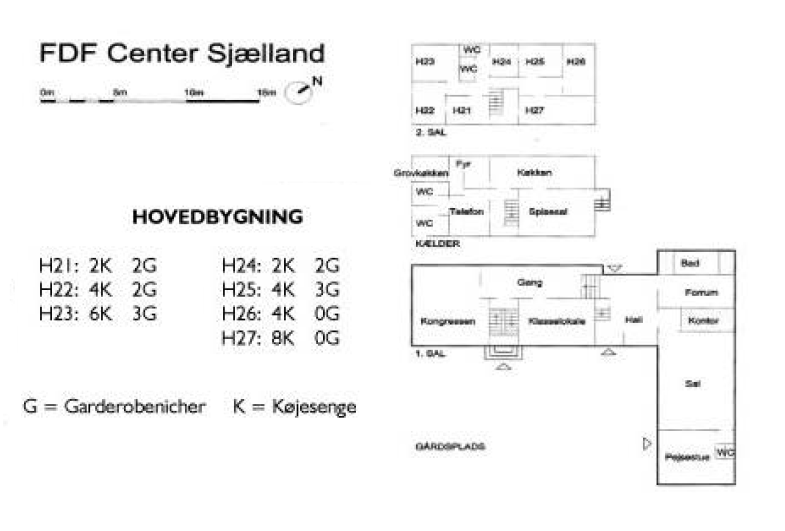
\includegraphics[width=\textwidth]{fig/Grundplan.png}
\end{center}
\end{figure}

\clearpage
\Overskrift{Mandag}
\section{Hyttebumser og KABS ankomst mandag}

\subsection*{Hyttetjek}
\begin{itemize}
\item Undersøg om ALT virker. Især ovne, kogeplader, køleskabe, frysere, toiletter, håndvaske og andre dyre maskiner.
\item Find ud af hvorvidt, der er septiktank eller kloak. Hvis der er septiktank, undersøg da hvordan lokummerne skyller. Hvis ikke vandet flyder perfekt ud, skal der bestilles slamsugning og det skal være med det samme!
\item Undersøg hvert rum for skader, såsom store huller i vægge eller manglende døre osv.
\item Tæl alt op i køkkenet. 
\item Husk foto hvis noget mangler.
\end{itemize}

\subsection{To do i de enkelte lokaler}
\begin{itemize}
\item Ølrum
	\begin{itemize}
	\item Modtage øl
	\item Få det bragt til ølrummet
	\item Sæt kasserne så de står sorteret efter type, det gør det hele meget nemmere senere.
	\item Øl-computer sættes op.
	\end{itemize}
\item Fest/spiserum	
	\begin{itemize}
	\item Musikanlæg sættes op på en måde så folk ikke umiddelbart kan smadre noget
	\item Tjanse-skema ophænges
	\item Ugeplan ophænges
	\end{itemize}
\item Sovesale
	\begin{itemize}
	\item Skilte ophænges på døre til tværholdene
	\item Forbudt-skilte ophænges på vektorernes døre
	\end{itemize}
\item Toiletter
	\begin{itemize}
	\item Der sættes papir på SAMTLIGE toiletter
	\item Sæbe på toiletterne
	\item Skilte med håndvask, drengtoilet og pigetoilet opsættes
	\end{itemize}
\item Generelt
	\begin{itemize}
	\item Resterende skilte hænges op
	\item Husk at tage billeder som dokumentation for hyttens renhed.
	\end{itemize}
\end{itemize}



\newpage
\section{Bussen}
\subsubsection*{\textbf{Ansvarlig:} \Hemorides}

Folk samles i tværhold, og sendes ind i bussen i tværhold. \\

Kryds alle russer af inden de går ind i bussen.
Ingen forlader bussen hvis de er krydset af.

Ring til hyttebumser/KABS når vi kører fra DTU.

\textbf{Varighed af turen:} lidt over en 1 time.

Spørg buschefføren (bus regler): Må vi bytte pladser? tissepause? Må vi drikke øl? Mikrofon brug.

Fortæl de små russere:
\begin{itemize}
  \item Vi skal til Center Sjælland
  \item Bussens faciliteter.
  \item Affald i poserne, ikke på gulvet\ldots
  \item Hvor lang tid tager turen?
  \item Vigtig: Broskål
  \item LEG eller DØ, så er I nogle champs!
\end{itemize}

\textbf{Drikkelse til turen:}  

\subsection*{Speeddating spørgsmål}
Tillægsspørgsmål: Bacon.
\begin{itemize}
  \item Hjemby og fødested
  \item Kollegie eller lejlighed?
  \item Remo eller mayo?
  \item Vil du helst være lam i højre side eller venstre side?
  \item Colgate eller Zendium?
  \item Vil du helst være lam eller gå på RUC?
  \item Store eller små fødder?
  \item Computer eller luksus?
  \item Øl eller cider?
  \item Hvorfor er du awesome?
  \item Sprødt eller blødt bacon?
  \item Brunetter eller blondiner?
  \item Cola eller pepsi? 
  \item Angelina Jolie eller Megan Fox? 
  \item Gyser eller komedie? 
  \item Bacon i strimler eller bacon i tern? 
  \item Hund eller kat? 
  \item A eller B menneske? 
  \item Tisse i bukserne eller kaste op på din mad? 
  \item Mayonaise som spyt eller remoulade som sved? 
  \item Orgasme hver 5. Minut eller aldrig orgasme?
  \item Intet hår eller 1 kubikmeter hår? 
  \item Vil du helst bryde i brand når du griner eller gå i opløsning når du græder? 
  \item Ingen ben eller ingen arme? 
  \item 1 meter højere eller 1 meter lavere? 
  \item Øre i fødderne eller mund på numse? 
  \item Bacon flettet eller bacon kurv? 
  \item Badeferie eller skiferie? 
  \item McDonalds eller BurgerKing? 
  \item Fisk eller Gajol? 
  \item Spanking eller fisting? 
  \item Sig 5 gode ting om kanelgifler 
  \item Koldskål eller faxekondi? 
  \item Hvilket dyr vil du helst være? 
  \item Forfra eller bagfra eller begge dele på samme tid? 
  \item Vil du helst spise din kebab som du har tisset i eller drikke en andens tis? 
  \item Vil du helst være usynlig eller kun flyve mod nord?
  \item Hvad er dit forhold til drager? 
  \item Hvad er din mest upassende scorereplik? 
  \item Hvad vil du helst, sluge et batteri eller leve resten af dit liv på Mors? 
  \item Krøller du eller folder du?
  \item Hvis du skulle have en 3. Arm, hvor skulle den så sidde? 
  \item Røv eller bryster? 
  \item Hvad vil du helst, være skaldet over hele kroppen eller aldrig blive klippet? 
  \item Hvad vil du helst, være i cølibat i 2 år eller uden internt i 2 år? 
  \item Hvad vil du helst, være blind eller RUC’er? 
  \item Rød læbepromade eller sprægte læber? 
  \item Hvad vil du helst, have evig racermave eller konstant kløe? 
  \item Hvad vil du helst, have lommelygter som hænder eller spande som fødder? 
  \item Hvad vil du helst, ikke have nogen hænder eller ikke have nogen kønsorganer 
  \item Hvad vil du helst, høre ”What does the fox say” på repeat, eller være Justin Biebers slave? 
  \item Hvad vil du helst, have permanent monobryn eller permanent have en bussemand hængende fra næsen? 
  \item Hvad vil du helst, have Amalie som datter eller som mor? 
  \item Hvad vil du helst, danse i stedet for at gå eller synge i stedet for at tale?
  \item Hvad vil du helst, have mos på tænderne eller permanent en rulleskøjte på den ene fod? 
\end{itemize}

\subsection*{Toiletrulleræs}
Højre side af bussen mod venstre side. En toiletrulle skal transporteres fra forrest i bussen til bagerst og tilbage igen, ved at blive rullet ud på vej ned og rullet ind på vej tilbage. Hvis papiret går i stykker skal man starte forfra. \\
Avanceret udgave: Toiletrullen skal rulles på kryds og tværs af midtergangen. 

\textbf{15 min før vi er der:} Nu er vi ved at være der! Når I går ud ad bussen, så tag jeres ting og gå hen til gårdspladsen og smide deres ting der.

\textbf{Når vi kommer hjem igen:} Vi ankommer til bygning 101 B eller E. \Hashtag{MadAuktion!}

\section{Velkomsttale}
\subsubsection*{\textbf{Ansvarlig:} \Farav }

Mine damer og herrer - velkommen til Center Sjælland!\\
Vi er nu trådt ind i år 2033. De sidste 20 år er der blevet kæmpet en dødelig krig over klodens sparsomme ølressourcer. Verdenen har været vidne til mange ubehagelige ting, og kun 8 lande er tilbage. De er:

\begin{itemize}
  \item Skotland
  \item Sydøstasien
  \item USA
  \item Ølympen
  \item Brasilien
  \item Vikingeland
  \item Den australske outback
  \item Egypten
\end{itemize}

Vi er samlet på dette sted for at finde den retmæssige verdenshersker, og for at fordele de resterende landområder imellem os. Og den eneste rigtige måde at gøre det på, er naturligvis ved at spille RISK!

I kampen om landene og de sidste ølressourcer vil i naturligvis få hjælp fra jeres vektorer og mig. Mit navn er Farav Ikmer, og jeg er KABS, hvilket står for Koordinator af Bachelor Studiestarten, og jeg læser Fysik og Nanoteknologi på 5. semester. Jeg er naturligvis lederen af Egypten.

\vspace{12pt}
\textbf{Præsentation af vektorer. Sig navn, retning, semester og lande\\
\clint \buddha \stive \hemorides \randildo \karla \mighty 
}\vspace{12pt}

I undrer jer uden tvivl over, hvorfor vi ikke skal have delt verdenshavene imellem os. Dette skyldes at de 7 fugtige områder bevogtes af tre vederstyggelige pirater, som tilfældigvis også har tilbudt at lave mad til os:

\vspace{12pt}
\textbf{Præsentation af hyttebumser. Sig navn, retning og semester\\
\Hyttebums{Pirates}
}\vspace{12pt}

I har sikkert bemærket at Karla og jeg har smukke neongule veste på. Det betyder at vi er ædru og har ansvar. Jeg er dagsansvarlig og skal sørge for at rusturen kører på skinner, og Karla er kørselsansvarlig og kan til enhver tid køre, hvis der bliver brug for det. Disse veste går på skift hver dag, og hvis I har problemer, kan man altid hive fat i en med vesten. Derudover har kørselsansvarlig et kamera, som alle med normaltfungerende balancesans meget gerne må låne.

\subsection*{Regler}
\begin{itemize}
  \item \textbf{Holdkæft-håndtegn} - Når hånden rækkes op tier man stille og rækker selv hånden op. Ingen snakker med hånden oppe.
  \item \textbf{Rygning} - Foregår udendørs. Skodder i spanden. Husk at vise hensyn hvis I ryger i en gruppe med ikke-rygere. 	
  \item \textbf{Smadrede ting} - Hvis man smadrer ting kontaktes dagsansvarlig.
  \item \textbf{Dansk lovgivning} - Gælder! Ingen stoffer, vold og hærværk. Hvis i har noget med så skal det afleveres i dag.
  \item \textbf{Drejebøger} - Hvis I finder en, så giv den til vektoren, der har tabt den - vedkommende kvitterer så med en øl. Lad være med at kigge i den, da det ødelægger turen.
  \item \textbf{Mobiltelefoner og ure} - skal blive i tasken - vi er her for at lære hinanden bedre at kende, og facebook er der også når I kommer hjem.
  \item \textbf{Badekar} - hvad er det? Tag bare, men husk at lægge ting på plads og passe på tingene. 
  \item \textbf{Musikcomputer} - Sæt i kø, ingen øl ved computeren. Det koster en øl at blive taget. Ikke pille ved volumen. Sæt ikke den samme sang i kø flere gange.
  \item \textbf{Badges} - finder man et, afleveres det til rette vedkommende, som så kvitterer med en øl
\end{itemize}

\subsection*{Praktisk info omkring hytten/turen}
\begin{itemize}
  \item Hvor sover man? (Ingen fest på sovesale)
  \item Hvor spiser man?
  \item Hvor skider man?
  \item Hvor leger man?
  \item Hvor går grunden til? (Gør det klart, at man ikke må forlade området)
  \item Ingen adgang skilte
  \item Vækning og morgenrejsning - sidste hold får toilettjansen!
  \item Tjanseskema og aktivitetsskema
  \item Førstehjælpskasse i køkkenet, skaf en vektor hvis der sker noget
\end{itemize}

\subsection*{Køkkenet}
\subsubsection*{\textbf{Ansvarlige:} \Hyttebums{Piraterne}}
\begin{enumerate}
  \item Hyttebumserne bestemmer alt
  \item Reglerne i køkkenet, madplanen, rushjælp til mad mm.
  \item Hvor man afleverer viskestykker / toiletpapir
  \item Vask hænder!
  \item Promiller i køkkenet
  \item Fodtøj
\end{enumerate}

\subsection*{Missionskort og RISK}
\subsubsection*{\textbf{Ansvarlig:} \Mighty}
Hver dag vil hvert hold få udleveret nogle missionskort, hvorpå en mission står skrevet samt hvor mange armeer den er værd (antal stjerner). Når man drager ud på en mission er det vigtigt man hiver fat i en voksen (vektor eller KABS), som kan godkende den forhåbentlig succesfulde mission. Armeerne benyttes til at erobre lande ved at holdet tager sine armeer og placere dem på de lande de vil erobre. Et land er først erobret, når holdet har flest armeer i pågældende land, dog må man ikke erobre et andet holds hjemland. Undervejs vil der også være drabelige kampe mellem holdene som også giver armeer. Det hold som tilsidst har erobret flest lande udnævnes som verdensherskere og vindere af RISK-spillet. \Hashtag{nemt} \\


\subsection*{Øl regler}
\subsubsection*{\textbf{Ansvarlig:}  \stive \hemorides \farav \mighty \buddha \randildo}
\begin{itemize}
  \item \textbf{Drik mellem mærkenrne} - \stive forklarer: når man åbner en øl er man tørstig, derfor er det selvfølgelig vigtigt, at man tager en ordentlig slurk af den lige til mellem mærkerne. Hvis det skulle ske at man drikker mere end mellem mærkerne er man tydeligvis meget tørstig, derfor kan man ligeså godt bunde. Hvis det omvendte skulle ske og man ikke kan drikke nok til mellem mærkerne er man ikke tørstig nok, derfor er det bedst for alle man bunder og starter forfra. Han demonstrere naturligvis undervejs og bunder!
  \item \textbf{Ølsjusk} - \hemorides forklarer og kommer til at spilde sin øl: man spilder naturligvis ikke sin øllebajser/cider, men hvis det skulle ske har man tydeligvis ikke drukket nok og derfor bunder man.
  \item \textbf{Buffalo} - \farav forklarer: tilbage i det vildeste vesten var en meget kendt cowboyder Bufallo Bill: kendt for sine vilde evner med en pistol og sin store kærlighed til øl og whiskey. Dengang i det vilde vesten sad pistolen altid ved højre hofte, så man hurtigt kunne komme til den og skyde hvem der nu var lidt træls. En dag Buffalo sad på hans stam saloon og havde fået serveret sin yndlings whiskey, en yderst exceptionel extra dry single malt whiskey fra Skotland, han sippede til med HØJRE HÅND. Uheldigvis for Buffalo braste en bandit ind af døren i samme øjeblik og skød vildt og voldsomt omkring sig. Buffalo forsøgte at trække sin pistol, men var simpelthen for langsom og nåede det ikke før en kugle gennemborer hans hjerte. Derfor drikker man ALTID med venstre hånd for at kunne nå sin pistol og forsvare sig, dog bunder man ALTID med højre, da man så kan benytte drikkegenstanden til kasteskyts og forsvare sig på den måde. Så hvis man skulle få øje på en person som drikker med højre hånd eller bunder med venstre råber man "BUFFALO!" og personen bunder en genstand.
  \item \textbf{Værktøjsregel} - \mighty forklarer værktøjsreglen mens Hæmorides prøver at åbne en øl, han failer hvorefter Mighty tager over og åbner. Hæmorides bunder og starter forfra. Værktøjsreglen: man har 3 forsøg til at åbne en øl med et hvilket som helst værktøj, man kan også udfordrer hinanden til at åbne en øl med et bestemt værktøj. Hvis der har været flere der har forsøgt køber de en genstand og bunder selvfølgelig også.
  \item \textbf{10 sekunder} - \buddha forklarer: man ønsker ikke at ens øl/cider skulle nå at blive flad, derfor har vi den vigtige 10 sekunders regel. Man har 10 sekunder til at finde kapslen og drikke mellem mærkerne. På den måde passer vi også på miljøet og slipper for at der flyder kapler over det hele. Miljøster passer selvfølgelig ekstra godt på miljøet og har derfor kun 5 sekunder til at finde kapslen.
  \item \textbf{Divine} - \buddha ser presset ud og \randildo diviner, samt forklare reglen. Personen man diviner skal give lov osv.
\end{itemize}

\textbf{HUSK} russerne på at druk er en gentlemans sport, alle skal have det sjovt!

\subsection*{Introduktion til ølsystem}
\textbf{Ansvarlig:} \Mighty
\begin{itemize}
  \item Russer får udleveret stregkodekort af deres vektorer
  \item Aflever fundne stregkodekort – belønning som sodavand/øl
  \item Hvordan skannersystemet virker
  \item Betaling
  \item Svind
\end{itemize}

\subsection*{Udfordrertrøjen} 
\begin{itemize}
  \item \mighty udfordrer \stive i at bunde en øl. Vinderen får udfordrerkappen og viser, hvad man skal skrive.
  \item Tusser findes i spisesalen
  \item Hvad der skal stå: \textbf{Navn, retning (forkortet) samt udfordring}
  \begin{itemize}
    \item Eksempelvis: Stive Irwin (Biotek) Master of Ølbunding
  \end{itemize}
\end{itemize}

\subsection*{Afrunding}
Og det var så krigens regler. I løbet af ugen vil I blive udsat for en masse sjove aktiviteter, og vi vil få besøg fra DTUs rektor og dekan, Polyteknisk Forenings bestyrelse samt IDA. Husk at I altid kan gå til dagsansvarlig eller en anden vektor hvis I har et spørgsmål. I kan nu følge med jeres vektor op til jeres værelser, og herefter er det tid til at få skabt noget nationalitetsfølelse og lavet nogle flag.



\input{tex/01-Mandag/Natløb.tex}

\clearpage
\Overskrift{Tirsdag}
\input{tex/02-Tirsdag/Krigsløb.tex}
\pagebreak

\section{Ingeniøropgave - Krigsmaskine}
\textbf{Ansvarlig:} \Buddha og \Hemorides

Russerne skal på 1 time lave en krigsmaskine i retningshold med de udleverede materialer. Der vurderes i point fra 1-5 hvor 1 er lavest og 5 er højest.
3. verdenskrig er udbrudt og I skal nu forsvare jeres retning ved at lave en krigsmaskine. På grund af krisen er der startet rationering på våben og materialer. Derfor har begrænsede materialer og må kun bruge dem til konstruktion af krigsmaskinen. Alle materialer fra naturen er naturligvis tilladt og må bruges. Det gælder om at skyde længst og der vurderes ud fra opfindsomhed, slagkraft, udførelse og bestikkelse. Hvert hold får udleveret:
\begin{itemize}
  \item 1 mælkekarton
  \item 1 kondom
  \item 1 tampon
  \item 10 elastikker
  \item 1 rulle sølvpapir
  \item 1 pakke grillspyd
  \item 1 pakke sugerør 
  \item 1 sort plastiksæk
  \item 1 rulle tape
  \item 5 meter snor
\end{itemize}

\subsection{Point}

\begin{table}[H]
\centering
\begin{tabu}{l *{7}{|C{1.4cm}}}
\specialrule{1pt}{0pt}{2pt}
\rowfont{\bfseries}
Kategori        & VBM & Elektro & P\&K & Biotek & Kemi & MatTek & Byg \\ \specialrule{1pt}{2pt}{1pt}
Slagkraft       & & & & & & & \\ \specialrule{.25pt}{1pt}{1pt}
Præcision       & & & & & & & \\ \specialrule{.25pt}{1pt}{1pt}
Opfindsomhed    & & & & & & & \\ \specialrule{.25pt}{1pt}{1pt}
Udførelse       & & & & & & & \\ \specialrule{.25pt}{1pt}{1pt}
Bestikkelse     & & & & & & & \\ \specialrule{1pt}{1pt}{0pt}
\end{tabu}
\end{table}

\subsection{Materialeliste}

\begin{itemize}
  \item 8 tomme mælkekartoner
  \item 8 kondomer
  \item 8 tamponer
  \item 80 elastikker
  \item 8 ruller sølvpapir
  \item 8 pakker grillspyd
  \item 8 pakker sugerør
  \item 1 rulle sorte affaldssække
  \item 8 ruller tape
  \item 40 meter snor
\end{itemize}
\pagebreak

\section{Mandeaften}

\textbf{Sted:} Græsplæne ude foran køkken. \\

\begin{tikzpicture}
   \draw[-, dashed] (-1,0) -- (0,0);
   \draw[|->, -latex] (0,0) -- (14,0);
   
   \draw[] (2,-0.1) -- (2,0.1);
   \draw (2,0) node[below=7pt,anchor=east,xshift=0,rotate=45] {Mande tale (15 min) - 20:00};
   
   \draw[] (4,-0.1) -- (4,0.1);
   \draw (4,0) node[below=7pt,anchor=east,xshift=0,rotate=45] {Pornonavne (15 min) - 20:15};
   
   \draw[] (6,-0.1) -- (6,0.1);
   \draw (6,0) node[below=7pt,anchor=east,xshift=0,rotate=45] {Smadre kål (20 min) - 20:30};
   
   \draw[] (8,-0.1) -- (8,0.1);
   \draw (8,0) node[below=7pt,anchor=east,xshift=0,rotate=45] {Vi råber (5 min) - 20:50}; 
   
   \draw[] (9,-0.1) -- (9,0.1);
   \draw (9,0) node[below=7pt,anchor=east,xshift=0,rotate=45] {Øl-budding stafet (30 min) - 20:55}; 
   
   \draw[] (11,-0.1) -- (11,0.1);
   \draw (11,0) node[below=7pt,anchor=east,xshift=0,rotate=45] {Kast fustager (20 min) - 21:25}; 
   
   \draw[] (13,-0.1) -- (13,0.1);
   \draw (13,0) node[below=7pt,anchor=east,xshift=0,rotate=45] {Lille prinsesse (15 min) - 21:45}; 
\end{tikzpicture}

\textbf{Mande tale:} \Farav holder mande talen. \\
\textbf{Pornonavne:} Vi finder pornonavne, man skal hedde resten af mandeaften \\
\textbf{Øl-budding staffet:} Vi løber ned, spiser øl-budding (plus løg og snackbacon) \\ 
\textbf{Kaster fustager:} Hvem kan kaste længest? \\
\textbf{Lille prinsesse:} Se næste side

\textbf{Husk:} Som rigtige gentlemen taber vi :-(

\textbf{Materiale liste}
\begin{itemize}
  \item Kål + Bat
  \item Dæk % så man kan sparke lidt til det
  \item Ting til at åbne øl med:
  \begin{itemize}
    \item Sav/hammer/værktøj
    \item Avis
    \item Krokketkugle
  \end{itemize}
  \item Plastik-kop til øl-budding (skal helst kunne tåle ca $50\,^{\circ}\mathrm{C}$ varmt vand)
\end{itemize}

\pagebreak
\textbf{Mine Herrer!}\\
- Vi er samlet her i dag, \underline{\textbf{UDEN KVINDER!}} Men hvorfor er vi det? Det er vi fordi vi har en historisk forpligtelse til at samles i patriarkiets hellige navn, for at praktisere den vigtigst og fornemste af de ting, der figurerer på den nærmest endeløse liste over ting, som mænd er i stand til, og som kvinder ikke er. Nej, vi snakker ikke om at køre bil, spille boldspil eller tage beslutninger. Vi snakker om at diskutere \textbf{VIGTIGE TING! (VIGTIGE TING! VIGTIGE TING!)}\\
- Det hele startede i år 336 f. Kr., hvor Alexander den Store samlede sine mænd og drog på erobringstogt \underline{\textbf{UDEN KVINDER}}. Men hvorfor gjorde han det? For at diskutere \textbf{VIGTIGE TING! (VIGTIGE TING! VIGTIGE TING!)}\\
- I år 58 f. Kr. gjorde en mand ved navn Julius Cæsar ham kunststykket efter. Han samlede ligeledes sine mænd og tog på erobringstogt \underline{\textbf{UDEN KVINDER}}. Men hvorfor gjorde han det? For at diskutere \textbf{VIGTIGE TING! (VIGTIGE TING! VIGTIGE TING!)}\\
- Så når vi frem til Jesus. Han var kendt som lidt af en blød sandalklædt metromand, der var god mod kvinder og dyr. Men da lokummet brændte samlede han sine desciple til nadver \underline{\textbf{UDEN KVINDER}} (fuck af, Dan Brown). Men hvorfor gjorde han det? For at diskutere \textbf{VIGTIGE TING! (VIGTIGE TING! VIGTIGE TING!)}\\
- Hunnerkongen Attila samlede i 430 sine mongolske frænder og tog ud for at plyndre og hærge og voldtage. Dette gjorde de \underline{\textbf{UDEN KVINDER}}. Men hvorfor gjorde de det? For at diskutere \textbf{VIGTIGE TING! (VIGTIGE TING! VIGTIGE TING!)}\\
- I år 600 samlede en mand ved navn Kong Arthur sine riddere omkring et bord, der havde samme smukke form som ølmaver og testikler. Det foregik naturligvis \underline{\textbf{UDEN KVINDER}}. Men hvorfor gjorde han det? For at diskutere \textbf{VIGTIGE TING! (VIGTIGE TING! VIGTIGE TING!)}\\
- I år 800 var det så vores hornklædte forgængere, vikingerne, der drak sig i mjød-hegnet, og tog ud i verden for at plyndre og hærge og voldtage. Det gjorde de \underline{\textbf{UDEN KVINDER}}. Men hvorfor gjorde de det? For at diskutere \textbf{VIGTIGE TING! (VIGTIGE TING! VIGTIGE TING!)}\\
- Så vil der ske om 600 år. Nemlig i år 1992, hvor den største mand af dem alle, Richard Møller Nielsen, samlede sine mænd og drog til Sverige for at vise hele verden hvordan rigtige mænd spiller fodbold. Ikke noget med fesne, langhårede, metroseksuelle, skabagtige driblekonger med hestetænder. Nej, rigtige mænd får bolden frem af banen ved at sparke HÅRDT og LANGT! Derfor drog han til Sverige uden angribere, og uden offensive midtbanespillere, men vigtigere endnu \underline{\textbf{UDEN KVINDER}}. Men hvorfor gjorde han det? For at diskutere \textbf{VIGTIGE TING! (VIGTIGE TING! VIGTIGE TING!)}\\
- Op gennem tiderne har kvinder mødtes uden mænd for at diskutere ting som strikkeopskrifter, balsamicoeddike, Paradise Hotel, nuancer af baige og hvilken håndcreme, der er bedst efter en lang dag med opvask og rengøring. Er det vigtige ting? (NEJ!!)\\
- Når mænd derimod igennem historien har mødtes \underline{\textbf{UDEN KVINDER}}, nøjagtig som vi i dag mødes og mænd ud i al fremtid vil mødes, bliver verdensordenen skabt, universets gåder afdækket, bajere drukket og peniser målt og sammenlignet. Men først og fremmest bliver der diskuteret..\\
\textbf{VIGTIGE TING!! VIGTIGE TING!! VIGTIGE TING!!}
\pagebreak

\pagebreak

\section{Dameaften}
\subsubsection*{\textbf{Ansvarlige:} \Randildo \& \Karla}

\textbf{Sted:} Pejsestuen \\

\begin{tikzpicture}
   \draw[-, dashed] (-1,0) -- (0,0);
   \draw[|->, -latex] (0,0) -- (14,0);
   
   \draw[] (2,-0.1) -- (2,0.1);
   \draw (2,0) node[below=7pt,anchor=east,xshift=0,rotate=45] {Introduktion (15 min) - 20:00}; 
   
   \draw[] (4,-0.1) -- (4,0.1);
   \draw (4,0) node[below=7pt,anchor=east,xshift=0,rotate=45] {Pige på DTU (5 min) - 20:15}; 
   
   \draw[] (5,-0.1) -- (5,0.1);
   \draw (5,0) node[below=7pt,anchor=east,xshift=0,rotate=45] {Kvindetalen + drinks (15 min) - 20:20}; 
   
   \draw[] (7,-0.1) -- (7,0.1);
   \draw (7,0) node[below=7pt,anchor=east,xshift=0,rotate=45] {Spørgsmål (20 min) - 20:35};
   
   \draw[] (9,-0.1) -- (9,0.1);
   \draw (9,0) node[below=7pt,anchor=east,xshift=0,rotate=45] {Perfekte Penis (20 min) - 20:55};

   \draw[] (11,-0.1) -- (11,0.1);
   \draw (11,0) node[below=7pt,anchor=east,xshift=0,rotate=45] {Føde børn (30 min) - 21:15};
   
   \draw[] (13,-0.1) -- (13,0.1);
   \draw (13,0) node[below=7pt,anchor=east,xshift=0,rotate=45] {Øve lille prinsesse (15 min) - 21:45}; 
   
   \draw[] (14,-0.1) -- (14,0.1);
   \draw (14,0) node[below=7pt,anchor=east,xshift=0,rotate=45] {Battle mod drengene (15 min) - 22:00}; 
\end{tikzpicture}

\subsection*{Introduktion}
Start: 20:00 \\
Tid: 15 minutter \\
Velkommen til pigeaften. Her skal vi bare hygge os helt vildt meget. Vi starter lige med en navnerunde hvor i kan fortælle lidt om jer selv:
\begin{itemize}
  \item Navn
  \item By
  \item Yndlings drink
  \item Fact om en selv
\end{itemize}

\subsection*{Pige på DTU}
\subsubsection*{\textbf{Ansvarlige:} \Karla}
Start: 20:15 \\
Tid: 5 minutter \\
Kære piger. \\
Jeg kan ikke forestille mig andet end at der i gymnasiet – eller hvor I ellers gik - skete rigtig mange ting; I udviklede jer selvfølgelig fagligt, men I lærte også meget om jer selv og menneskerne omkring jer. Det vil også ske på DTU. Det vil virkelig gøre mig glad, hvis det lykkes os at give jer den bedst mulige start på alle de her nye ting. Vi har jo været i gennem meget af det samme, så brug os, spørg os til råds om hvad end I har på hjertet. For der sker meget nyt. \\
Én af de ting I skal være forberedt på, og som sandsynligvis vil være nyt for de fleste af jer, er det markante overtal af drenge, I hele tiden vil være omgivet af. Og I kender dem – de kan sku godt være lidt liderlige og være det lidt hele tiden. Så tænk på jeres ry. I skal ikke blive skræmt, tage kyskhedsbælte på og smide nøglen væk, men de fleste af jer skal sandsynligvis være her i fem år, så pas på jer selv. Der kommer massere af muligheder for at slå jer løs. (Det gælder om at være glad i det lange løb :-) ).

\subsection*{Kvindetalen + drinks}
\subsubsection*{\textbf{Ansvarlige:} \Randildo}
Start: 20:20 \\
Tid: 15 minutter \\
Der serveres drinks inden talen begynder. \\

\subsection*{Spørgsmål}
Start: 20:35 \\
Tid: 20 minutter \\
Hver rus får en hvid serviet og en grøn serviet. Hvid serviet er negativ, grøn serviet er positiv. Servietten rækkes i vejret som svar på spørgsmålene som vektorerne stiller.

\begin{itemize}
  \item Hvem har en kæreste?
  \item Hvem har bare en lækker mand?
  \item Hvem har et sted at bo?
  \item Hvem kan godt lide at gå i kjoler?
  \item Hvem kan ridde?
  \item Hvem har malket en ko?
  \item Hvem har gået på STX?
  \item Hvem har gået på HTX?
  \item Hvem kan lave en fransk fletning?
  \item Hvem har været på en andet kontinent?
  \item Hvem har haft et sabbatår?
  \item Hvem kommer fra Jylland?
  \item Hvem kommer fra Sjælland?
  \item Hvem kommer fra Fyn?
  \item Hvem kan slikke på deres egen nipple? (prøv hvis stemningen er til det)
  \item Hvem har været sammen med deres kæreste i mere end 2 år?
  \item Var det nemt at finde kostume?
  \item Hvem er til storbyferie?
  \item Hvem er til badeferie?
  \item Hvem er til aktive ferier?
  \item Hvem er romantikere?
  \item Bliver mænd lækrere i jakkesæt? (glæd jer til årsfest)
\end{itemize}

\subsection*{Den perfekte penis}
Start: 20:55\\
Tid: 20 minutter\\
Introduktion: \randildo
Man får en klump trylledej hver og skal forme den perfekte penis.\\
Vi bruger den samme trylledej som fra natløbet mandag.\\

\subsection*{Føde børn}
Start: 21:15 \\
Tid: 30 minutter \\
Introduktion af \hspace{.1em} \Hyttebums{Jack}og\hspace{.2em} \Hyttebums{Turn-On} \\
Man ligger som om man skal føde, har en cykelslange mellem benene og skyder en bamse af sted. En anden pige står for at gribe den mellem armene som en jordmoder. 

\subsection*{Øve lille prinsesse}
Start: 21:45 \\
Tid: 15 minutter \\
Øve lille prinsesse efter sangbogen samt finde på flere vers, så vi kan slå drengene. Pigerne vinder.

\subsection*{Lille prinsesse – battle mod drengene}
Start: 22:00 \\
Tid: Så lang tid den kan fortsættes \\
Battle mod drengene i lille prinsesse. \\
Pigerne skal vinde (have skrevet nogen på forhånd)
\begin{itemize}
  \item Jeg kan dig ikke føle
  \item Du kom jo alt for hurtigt
  \item Din bror var 3 gange større
  \item Hvis der kommer noget om søster: hun er jo længe afdød
  \item Gå hjem til plastikdukken
  \item Behøver jeg sige mere
\end{itemize}

\subsection*{Materialeliste:}
\begin{itemize}
  \item Hvide servietter
  \item Grønne servietter
  \item 2-3 Cykelslanger
  \item 2-3 Bamse-lignende ting
  \item 6L danskvand
  \item 1 flaske Hyldeblomstsaft
  \item 6 lime
  \item 2 flaske vodka
\end{itemize}

\pagebreak
Ærede kvinder, mine Damer! \\
Vi er her samlet her i dag som ligesindede, \underline{\textbf{UDEN MÆND}}. Og hvorfor er vi det? Det er vi fordi vi har en historisk pligt til at samles for at praktisere én af den uendelige mængde af ting, som vi kvinder gør bedre end mænd. Og hér snakker jeg ikke om evnen til at dufte godt, være syg uden at klynke, rydde op i køkkenet UNDER madlavning eller utallige andre kompetencer såsom evnen til at koncentrere sig i længere tid. Jeg taler heller ikke om evnen til at lave en matematikaflevering, mens vi taler i telefon og samtidig får klaret dagens knibeøvelser. Nej, jeg snakker om evnen til at diskutere \textbf{VIGTIGE TING!} I år 0 blev det lille Jesus barn født af ingen ringere end selveste Jomfru Maria; En fantastisk kvinde, hun klarede det hele selv, \underline{\textbf{UDEN MÆND}}. Men hvordan gjorde hun det? Jo, hende og Gud havde diskuteret \textbf{VIGTIGE TING!} Mændenes historie fyldt med blod, og meningsløs vold og død. Det var aldrig gået så galt, hvis blot vi havde levet \underline{\textbf{UDEN MÆND!}} Eksemplerne er talrige: Alexander den Stores erobringstogt i år 336 f. kr., Hunnerkongen Attilas togt i 430 med plyndring og voldtægt, Vikingerne, Napoleon, Stalin, Hitler. Alle disse timer og liv spildt, blot fordi mænd ikke kan finde ud af at diskutere \textbf{VIGTIGE TING!} Snakker vi derimod kvindelige regenter, så har der, for hver eneste konge igennem historien været en dronning ved hans side, men når man kigger nøje efter vil man opdage, at der ikke for hver dronning har været en konge! Jeg taler om Kleopatra, Elizabeth I og selvfølgelig om Danmarks to Margrether’; Dronninger som har formået at samle Norden, lede Nationen og regere over folket og de har gjort det \underline{\textbf{UDEN MÆND}}. Men hvordan gjorde de det? Ved at diskutere \textbf{VIGTIGE TING!} På trods af, at mændene dræber og kvinderne skaber, så er det alligevel mændenes bedrifter som har fået størst genklang i historien. Derfor vil vi i dag gerne ære to kvinder, som er blevet overset, men som har banet vejen for, at vi sidder her i dag, nemlig: Agens Klingberg og Betzy Meyer, der i 1897 blev Danmarks første kvindelige ingeniører. Det gjorde de \underline{\textbf{UDEN MÆND, PÅ TRODS AF MÆND}} og de gjorde det ved at diskutere \textbf{VIGTIGE TING!} Når mænd mødes, uden kvinder, så bruger de tiden på at diskutere ting såsom, hvis prut der lugter mest, hvem der er kommet længst i Command and Conquer, hvem der har håneretten i ølrisk eller hvem der er den bedste James Bond. Er det vigtige ting? (\textbf{NEJ!}) Vi kvinder sidder IKKE og klør os i skridtet, piller næse og finder navlefnuller uden at kunne overskue at rejse os op for at hente en bajer, \textbf{NEJ!}, når kvinder mødes, \underline{\textbf{RIGTIGE KVINDER}}, nøjagtigt som vi gør her i aften og som vi vil mødes i al fremtid, bliver relationer skabt, verdenssituationen vendt, problemer løst, skønhed udforsket og viden delt! Der bliver sammenlignet outfits, snakket om penislængder, og analyseret sms’er. Men først og fremmest så bliver der diskuteret.. \textbf{VIGTIGE TING! VIGTIGE TING! VIGTIGE TING!}

\pagebreak


\clearpage
\Overskrift{Onsdag}
\input{tex/03-Onsdag/DTU-løb.tex}

\section{IDA kommer}
\vspace{-3.35em}
\subsection*{\hspace{11.5em} ... når du piller ved hende {\tt ;)}}

\randildo, \farav, og \hemorides flytter borde og stole så der er klar til IDA.

\newpage
\section{FN konventionen}
\textbf{Ansvarlig:} \Farav

Der er FN topmøde, og verdens nationer er samlet for at smide et land ud af FN, så de andre lande får mere magt. Hvert land skal argumentere for, at et andet land skal ekskluderes, og til sidst bestemmes det, hvem der har holdt den bedste tale. 

\begin{center}
\begin{tabular}{l | l}
\specialrule{1pt}{1pt}{0pt}
\textbf{Hvem holder tale} & \textbf{Hvad taler de om}\\ \specialrule{1pt}{1pt}{0pt}
\Hb{Piraterne} & Holder tale om Egypten \\\specialrule{.25pt}{1pt}{1pt}
\cfarav{Egypten} & Holder tale om Skotland \\\specialrule{.25pt}{1pt}{1pt}
\cmighty{Skotland} & Holder tale om 'Murica \\\specialrule{.25pt}{1pt}{1pt}
\cclint{'Murica} & Holder tale om Ølympen \\\specialrule{.25pt}{1pt}{1pt}
\chemorides{Ølympen} & Holder tale om  Sydøstasien \\\specialrule{.25pt}{1pt}{1pt}
\cbuddha{Sydøstasien} & Holder tale om Brasilien \\\specialrule{.25pt}{1pt}{1pt}
\crandildo{Brasilien} & Holder tale om Vikingeland\\\specialrule{.25pt}{1pt}{1pt}
\ckarla{Vikingeland} & Holder tale om Australien\\\specialrule{.25pt}{1pt}{1pt}
\cstive{Australien} & Holder tale om Piraterne\\ \specialrule{1pt}{1pt}{0pt}
\end{tabular}
\end{center}


\subsection*{Grundlag for talerne}
Grundlag for hvorfor de forskellige lande skal ekskluderes fra FN (for selv at få mere magt):\\

\textbf{Egypten}, De er forhistoriske og håbløst umoderne, og de brugte slaver til at udføre det hårde arbejde.\\
\textbf{Skotland}, De tror på Loch Ness uhyret, er klamme og spise fåreindvolde. Og sækkepiber.\\
\textbf{'Murica}, de laver ikke andet end at skyde hinanden og sagsøge McDonalds fordi de er blevet tykke. \\
\textbf{Ølympen}, de tror de er guder, men i virkeligheden burde de bare få styr på deres økonomi.\\
\textbf{Sydøstasien}, de er alt for fredelige til at være med til krig. \\
\textbf{Brasilien}, de er elendige til fodbold og de tror at samba løser alle problemer. \\
\textbf{Vikingeland}, de er uciviliserede og horer og plyndrer og voldtager alt. \\
\textbf{Australien}, det er så langt væk, at de praktisk set ikke er en del af verden, og så er der alt for mange slanger og kæmpe edderkopper.\\
\textbf{Piraterne}, de er upassende, vasker aldrig hænder og lugter generelt dårligt.\\
\textbf{Generelt}, man må gerne rose sig selv.


\subsection*{Udførelse}
Russerne får at vide, hvem de skal holde tale om til frokost, og så kan de benytte eftermiddagen på at forberede sig. Talerne afholdes efter aftensmaden. Der stilles en ``talerstol'' op inden talerne. Der er medbragt hammer og noget at slå på så FN-delegationen kan bibeholde roen hvis nødvendigt.\\
KABS og vektorer sørger for at talerækken overholdes.

Hvert hold skiftes til at gå op til talerstolen for at fremsige deres mere eller mindre skrevne tale.\\
Der lægges vægt på at det holdes upersonligt - altså går man efter et land, ikke en mand. Talerne skal vare i ca. 5 minutter, og der gives point efter udførelse, opfindsomhed, sjovhed og bestikkelse. Der gives point fra 1-10. Afslutningsvist: FN-delegationen kårer den sjoveste tale og gevinst er tre armeér. Ingen nationer ekskluderes.

\begin{center}
\begin{tabular}{l|c} \specialrule{1pt}{1pt}{0pt} 
\textbf{Land} & \textbf{Point}\\ \specialrule{1pt}{1pt}{0pt}
Piraterne   & \\\specialrule{.25pt}{1pt}{1pt}
Egypten     & \\\specialrule{.25pt}{1pt}{1pt}
Skotland    & \\\specialrule{.25pt}{1pt}{1pt}
'Murica     & \\\specialrule{.25pt}{1pt}{1pt}
Ølympen     & \\\specialrule{.25pt}{1pt}{1pt}
Sydøstasien & \\\specialrule{.25pt}{1pt}{1pt}
Brasilien   & \\\specialrule{.25pt}{1pt}{1pt}
Vikingeland & \\\specialrule{.25pt}{1pt}{1pt}
Australien  & \\ \specialrule{1pt}{1pt}{0pt}
\end{tabular}
\end{center}

\subsection{Materialeliste}
\begin{itemize}
\item 6 Udprintede FN-logoer til at sætte på vestene, hvoraf 3 er A4 og 3 er A5.
\item 20 sikkerhedsnåle til at sætte det udprintede på vestene
\item Papir og skriveredskaber til alle
\item Hammer
\item Noget at slå på med hammeren (evt. et stykke træ)
\item Improviseret talerstol - evt. et omvendt bord.

\end{itemize}

\clearpage
\Overskrift{Torsdag}
\section{Festaften}
Russerne arrangerer selv festaften. Vi hænger skemaer op med tjanser i pejsestuen torsdag morgen. Dagsansvarlige annoncerer til morgenrejsning torsdag, at russerne selv skal skrive sig på.

\begin{enumerate}
\item Oppyntning - Ansvarlig: \Randildo \& \Clint
\item Bar - Ansvarlig: \Stive \& \Hemorides
\item Madlavning - Ansvarlig: \Hyttebums{Piraterne}
\item Oprydning - Ansvarlig: \Farav \& \Mighty
\item Underholdning - Ansvarlig: \Karla \& \Buddha
\end{enumerate}

\subsection*{Oppyntning - 10 russer}
\subsubsection*{Ansvar: \Randildo \& \Clint}
Dække bord, pynte borde og vægge. Der skal indkøbes:
\begin{itemize}
\item Duge
\item Balloner
\item Serpentiner
\item Fyrfadslys
\item Sølvpapir til lysestager
\item Tape
\end{itemize}

\subsection*{Bar - 10 russer}
\subsubsection*{Ansvar: \Stive \& \Hemorides}
Der bliver købt ind til 2 slags drinks. Der bliver lavet streglister så russerne betaler over ølregning individuelt. Baransvarlige skal altid være i baren, således det ikke stikker af. Fif: Vent med at blande det hele. Der skal indkøbes:
\begin{itemize}
  \item Vodka + Saftevand
  \item Rom + Cola
  \item Plastglas 400 stk.
  \item Sugerør 400 stk.
\end{itemize}

\subsection*{Madlavning - 8 russer}
\subsubsection*{Ansvar: \Hyttebums{De glade Sømænd}}
\Hyttebums{Piraterne} winger den

\subsection*{Oprydning efter aftensmad - 11 russer}
\subsubsection*{Ansvar: \Farav \& \Mighty}
Opsætning til B14s show og rengøring af Kongressen, så vi ikke behøver at gøre det fredag.\\
Almindelig oprydning og hjælp til \Hyttebums{Piraterne} i køkkenet efter maden \Hashtag{oprydningsfist}. 

\subsection*{Underholdning - 10 russer}
\subsubsection*{Ansvar: \Karla \& \Buddha}
Russerne planlægger selv aktivitet. Ideer hertil:
\begin{itemize}
  \item Sedler under tallerknerne  med ``opgaver'' under maden
  \item Et teaterstykke
  \item En dans
  \item En tale
  \item En leg - Fx en fra hvert hold skal stille en person
  \item Gæt og grimasser \Hashtag{GørNogetUpassende}
\end{itemize}

\subsection{Afsløring af Tip en Vektor}

\begin{table}[H]
\centering
\begin{tabu}{L{11.7cm} L{3.5cm}}\specialrule{1pt}{0pt}{2pt}
\rowfont{\bfseries} Spørgsmål & Svar \\ \specialrule{1pt}{2pt}{1pt}
1) Hvem valgte at bunde en masse Fernet Branca, hvorefter personen teleportede sig fra Rødby til et poolbord i S-huset? & \hemorides \\ \specialrule{.25pt}{1pt}{1pt}
2) Hvem har brugt over 300 euro på sit kostume? & \mighty \\ \specialrule{.25pt}{1pt}{1pt}
3) Hvem gemte sig under klapsæderne i 35 min. i et tog for at spare penge? & \farav \\ \specialrule{.25pt}{1pt}{1pt}
4) Hvem har sovet udenfor DTU-skiltet efter en aften i kælderbaren og herremiddag, uden at kunne huske det dagen efter? & \buddha \\ \specialrule{.25pt}{1pt}{1pt}
5) Hvem har haft blå mærker hele vejen op ad begge ben fordi personen kravlede i bjælker på forberedelsestur? & \karla \\ \specialrule{.25pt}{1pt}{1pt}
6) Hvem har snavet samtlige af sine retningsvektorer? & \randildo \\ \specialrule{.25pt}{1pt}{1pt}
7) ”Hvad?! Jeg har aldrig gjort noget dumt” & \Hyttebums{Elizabeth} \\ \specialrule{.25pt}{1pt}{1pt}
8) Hvem stod af natbussen for at kaste op, for dernæst at erfare, der ikke kom flere busser? & \clint \\ \specialrule{.25pt}{1pt}{1pt}
9) Hvem har de korteste shorts? & \clint \\ \specialrule{.25pt}{1pt}{1pt}
10) Hvem valgte at tage en en-mands brandert i Minttu på forberedelsesturen? & \Hyttebums{Turn-On} \\ \specialrule{.25pt}{1pt}{1pt}
11) Hvem valgte at kalde max. 2 stykker tøj en aften på forberedelsesturen? & \Hyttebums{Swallows} \\ \specialrule{.25pt}{1pt}{1pt}
12) Hvem kan åbne svælget og bunde hurtigst? & \stive \\ \specialrule{.25pt}{1pt}{1pt}
13) Hvem er bedst til at spule på kommando? & \buddha \\ \specialrule{.25pt}{1pt}{1pt}
14) Hvis bare røv blev spanket i kælderbaren? & \stive \\ \specialrule{.25pt}{1pt}{1pt}
15) Hvem er bedst til kiks? & \karla \\ \specialrule{.25pt}{1pt}{1pt}
16) Hvis lægge vejer, ifølge ham selv, 40kg tilsammen? & \mighty \\ \specialrule{.25pt}{1pt}{1pt}
17) Hvem er bange for fødder? & \Hyttebums{Turn-On} \\ \specialrule{.25pt}{1pt}{1pt}
18) Hvem er den bedste morgen-boller? & \Hyttebums{Turn-On} \\ \specialrule{.25pt}{1pt}{1pt}
19) Hvilket hold vandt RISK på forberedelsesturen? & \farav, \buddha, \randildo \& \clint \\ \specialrule{.25pt}{1pt}{1pt}
20) Hvem spulede ikke på RISK-aften på forberedelsesturen? & \buddha \\ \specialrule{.25pt}{1pt}{1pt}
21) Hvem blev gagget af en gærpenis? & \stive \\ \specialrule{.25pt}{1pt}{1pt}
22) Hvem kan ikke finde ud af alfabetet? & \hemorides \\ \specialrule{.25pt}{1pt}{1pt}
23) Hvem blandt vektorerne/hyttebumZ/KABS er holdets spassere? & \hemorides \& \mighty \\ \specialrule{1pt}{1pt}{0pt}
\end{tabu}
\end{table}

\clearpage
\Overskrift{Fredag}
\input{tex/05-Fredag/Rengøring.tex}
\section{Pizzalister}
Vi ringer til La Sosta på 45 87 06 16 og bestiller pizzaer til alle i bussen. Alle pizzaer koster 50 kr, som betales med det samme, kontant eller mobile pay. \Stive sørger for at notere bestillinger og modtage penge samt ringe til La Sosta, når alle har noteret pizza. Der kan vælges mellem følgende pizzaer:
\begin{itemize}
\item F1: tomat, ost og skinke
\item F5: tomat, ost, kødsauce og løg
\item F7: tomat, ost, skinke og pepperoni
\item F9: tomat, ost, shawarma, salat og dressing
\end{itemize}

\begin{table}[H]
\centering
\begin{tabu}{L{8cm}|L{3cm}|L{3cm}}\specialrule{1pt}{0pt}{2pt}
\rowfont{\bfseries} Navn & Pizza nr. & Betalt   \\ \specialrule{1pt}{2pt}{1pt}
\cfarav{Egypten - Farav Ikmer}              & F1 & \\ \specialrule{.25pt}{1pt}{1pt}
Morten Bondorf Gerdes (MatTek)              & & \\ \specialrule{.25pt}{1pt}{1pt}
Sajeel Hussain (Elektro)                    & & \\ \specialrule{.25pt}{1pt}{1pt}
Annemette Ringsted (BioTek)                 & & \\ \specialrule{.25pt}{1pt}{1pt}
Anita Pedersen (Miljø)                      & & \\ \specialrule{.25pt}{1pt}{1pt}
Søren Bundgård (P\&K)                       & & \\ \specialrule{.25pt}{1pt}{1pt}
William Gundtorp (Kemi)                     & & \\ \specialrule{1pt}{1pt}{1pt}
\ckarla{Vikingeland - Karla K. Kløvehjerte} & F9 & \\ \specialrule{.25pt}{1pt}{1pt}
Lasse Thunbo (Byg)                          & & \\ \specialrule{.25pt}{1pt}{1pt}
Magnus Als (Miljø)                          & & \\ \specialrule{.25pt}{1pt}{1pt}
Sebastian Dessen (Elektro)                  & & \\ \specialrule{.25pt}{1pt}{1pt}
Sophie Natasha Silberbrandt (MatTek)        & & \\ \specialrule{.25pt}{1pt}{1pt}
Vanessa Niknazmanesh (BioTek)               & & \\ \specialrule{.25pt}{1pt}{1pt}
Alexander Neergård Bissen (Byg)             & & \\ \specialrule{.25pt}{1pt}{1pt}
Morten Harboe (Kemi)                        & & \\ \specialrule{1pt}{1pt}{1pt}
\crandildo{Brasilien - Randildo Bailando}   & & \\ \specialrule{.25pt}{1pt}{1pt}
Jeppe Sode Rung (BioTek)                    & & \\ \specialrule{.25pt}{1pt}{1pt}
Nicklas Nielsen (P\&K)                      & & \\ \specialrule{.25pt}{1pt}{1pt}
Morten Rydberg Wahlgreen (MatTek)           & & \\ \specialrule{.25pt}{1pt}{1pt}
Mette Torsberg Møller (Miljø)               & & \\ \specialrule{.25pt}{1pt}{1pt}
Peter Iwer Hoedt Karstensen (Elektro)       & & \\ \specialrule{.25pt}{1pt}{1pt}
Natasja Emilie Buchholdt (Byg)              & & \\ \specialrule{1pt}{1pt}{1pt}
\cclint{'Murica - Clint Hardwood}           & F1 & \\ \specialrule{.25pt}{1pt}{1pt}
Joachim Holm Knudsen (P\&K)                 & & \\ \specialrule{.25pt}{1pt}{1pt}
Josephine Byskov Tønder (MatTek)            & & \\ \specialrule{.25pt}{1pt}{1pt}
Karen Marie Jørgensen (BioTek)              & & \\ \specialrule{.25pt}{1pt}{1pt}
Rasmus Lykke Mortensen (Kemi)               & & \\ \specialrule{.25pt}{1pt}{1pt}
Christian Berg Jacobsen (Elektro)           & & \\ \specialrule{.25pt}{1pt}{1pt}
Morten Højen Kristiansen (Miljø)            & & \\ \specialrule{1pt}{1pt}{0pt}
\end{tabu}
\end{table}

\begin{table}[H]
\centering
\begin{tabu}{L{8cm}|L{3cm}|L{3cm}}\specialrule{1pt}{0pt}{2pt}
\rowfont{\bfseries} Navn & Pizza nr. & Betalt   \\ \specialrule{1pt}{2pt}{1pt}
\cstive{Australien - Stive Irwin}           & & \\ \specialrule{1pt}{1pt}{1pt}
Camilla Christiane Jakobsen (Miljø)         & & \\ \specialrule{.25pt}{1pt}{1pt}
Frederik Munck (Byg)                        & & \\ \specialrule{.25pt}{1pt}{1pt}
Johnny Martin Wanchai Seehuusen (Elektro)   & & \\ \specialrule{.25pt}{1pt}{1pt}
Oktay Ipek (Kemi)                           & & \\ \specialrule{.25pt}{1pt}{1pt}
Anders Dalsgård Melander (MatTek)           & & \\ \specialrule{.25pt}{1pt}{1pt}
Bjarke Dalhoff Christensen (P\&K)           & & \\ \specialrule{1pt}{1pt}{1pt}
\cmighty{Skotland - Mighty O'Long-John}     & & \\ \specialrule{.25pt}{1pt}{1pt}
Christian Vestbjerg (P\&K)                  & & \\ \specialrule{.25pt}{1pt}{1pt}
Emil Nørgaard Strøm (MatTek)                & & \\ \specialrule{.25pt}{1pt}{1pt}
Lars Chr. Vindfelt Jensen (BioTek)          & & \\ \specialrule{.25pt}{1pt}{1pt}
Malina Benedicte Mølmer (Kemi)              & & \\ \specialrule{.25pt}{1pt}{1pt}
Maria  Rotne Bessman (Byg)                  & & \\ \specialrule{.25pt}{1pt}{1pt}
Nikola Milanovic (Vand)                     & & \\ \specialrule{1pt}{1pt}{1pt}
\chemorides{Ølympen - Hæmorides af Ølympen} & F9 & \\ \specialrule{.25pt}{1pt}{1pt}
Thorbjørn Anker Sørensen(Kemi)              & & \\ \specialrule{.25pt}{1pt}{1pt}
Rikke Andersen (Byg)                        & & \\ \specialrule{.25pt}{1pt}{1pt}
Nick Hashan Thanthrige (Elektro)            & & \\ \specialrule{.25pt}{1pt}{1pt}
Tanya Teglbjærg (BioTek)                    & & \\ \specialrule{.25pt}{1pt}{1pt}
Gisli Tomas Gudjonsson (P\&K)               & & \\ \specialrule{.25pt}{1pt}{1pt}
Markus Mogensen Henriksen (Elektro)         & & \\ \specialrule{.25pt}{1pt}{1pt}
\cbuddha{Sydøstasien - Buddha Karma Sutma}  & & \\ \specialrule{.25pt}{1pt}{1pt}
Josefine Hvarregård Andersen (Kemi)         & & \\ \specialrule{.25pt}{1pt}{1pt}
Ingvi Örnolfsson (P\&K)                     & & \\ \specialrule{.25pt}{1pt}{1pt}
Sebastian Bov\'{e} Wagner (Elektro)         & & \\ \specialrule{.25pt}{1pt}{1pt}
Katja Kaastrup (BioTek)                     & & \\ \specialrule{.25pt}{1pt}{1pt}
Markus Pai Sørensen (Byg)                   & & \\ \specialrule{.25pt}{1pt}{1pt}
Sebastian Rosenquist (MatTek)               & & \\ \specialrule{.25pt}{1pt}{1pt}
Kristian Revsbech (Elektro)                 & & \\ \specialrule{1pt}{1pt}{0pt}
\end{tabu}
\end{table}

\clearpage
\Overskrift{Øvrigt}
\section{RISK reglerne}
Hvert hold får udleveret 5 missionskort ved ankomst, missionerne kan være alt fra at bunde en sodavand over kidnapning af hyttebumser til at vinde udfordrerkappen. Derudover uddeles 5 nye missionskort hver morgen. Ved udførelse af en mission, skal en voksen være til stede for at godkende. På hvert kort er der et antal stjerner, som angiver hvor mange armeer, man får for udførelse af missionen. Armeerne er i dette tilfælde farvede knappenåle, som placeres i et land på RISK-kortet, som bliver hængt op i spisesalen og som ses på figur \ref{fig:RISK}. Der uddeleles desuden armeer til vinderne af natløb, krigsløb og taler. Regler:
\begin{itemize}
  \item Armeer må ikke placeres i nogens hjemland - disse er fredet
  \item Armeer kan frit placeres - der er ikke krav om at man skal støde op til et land for at angribe
  \item Det hold med flest armeer i et land ejer landet
  \item Man må ikke flytte en arme efter den er placeret
  \item Det er udelukkende de voksne der må sætte nåle i brættet
  \item Det er absolut forbudt at pille ved brikkerne, også når vektorerne ikke kigger
\end{itemize}
De sidste missioner skal være udført torsdag aften inden aftensmaden, og vinderen \Hashtag{verdensherskeren} kåres efter hovedretten - præmien er badges.

\begin{figure}[H]
\centering
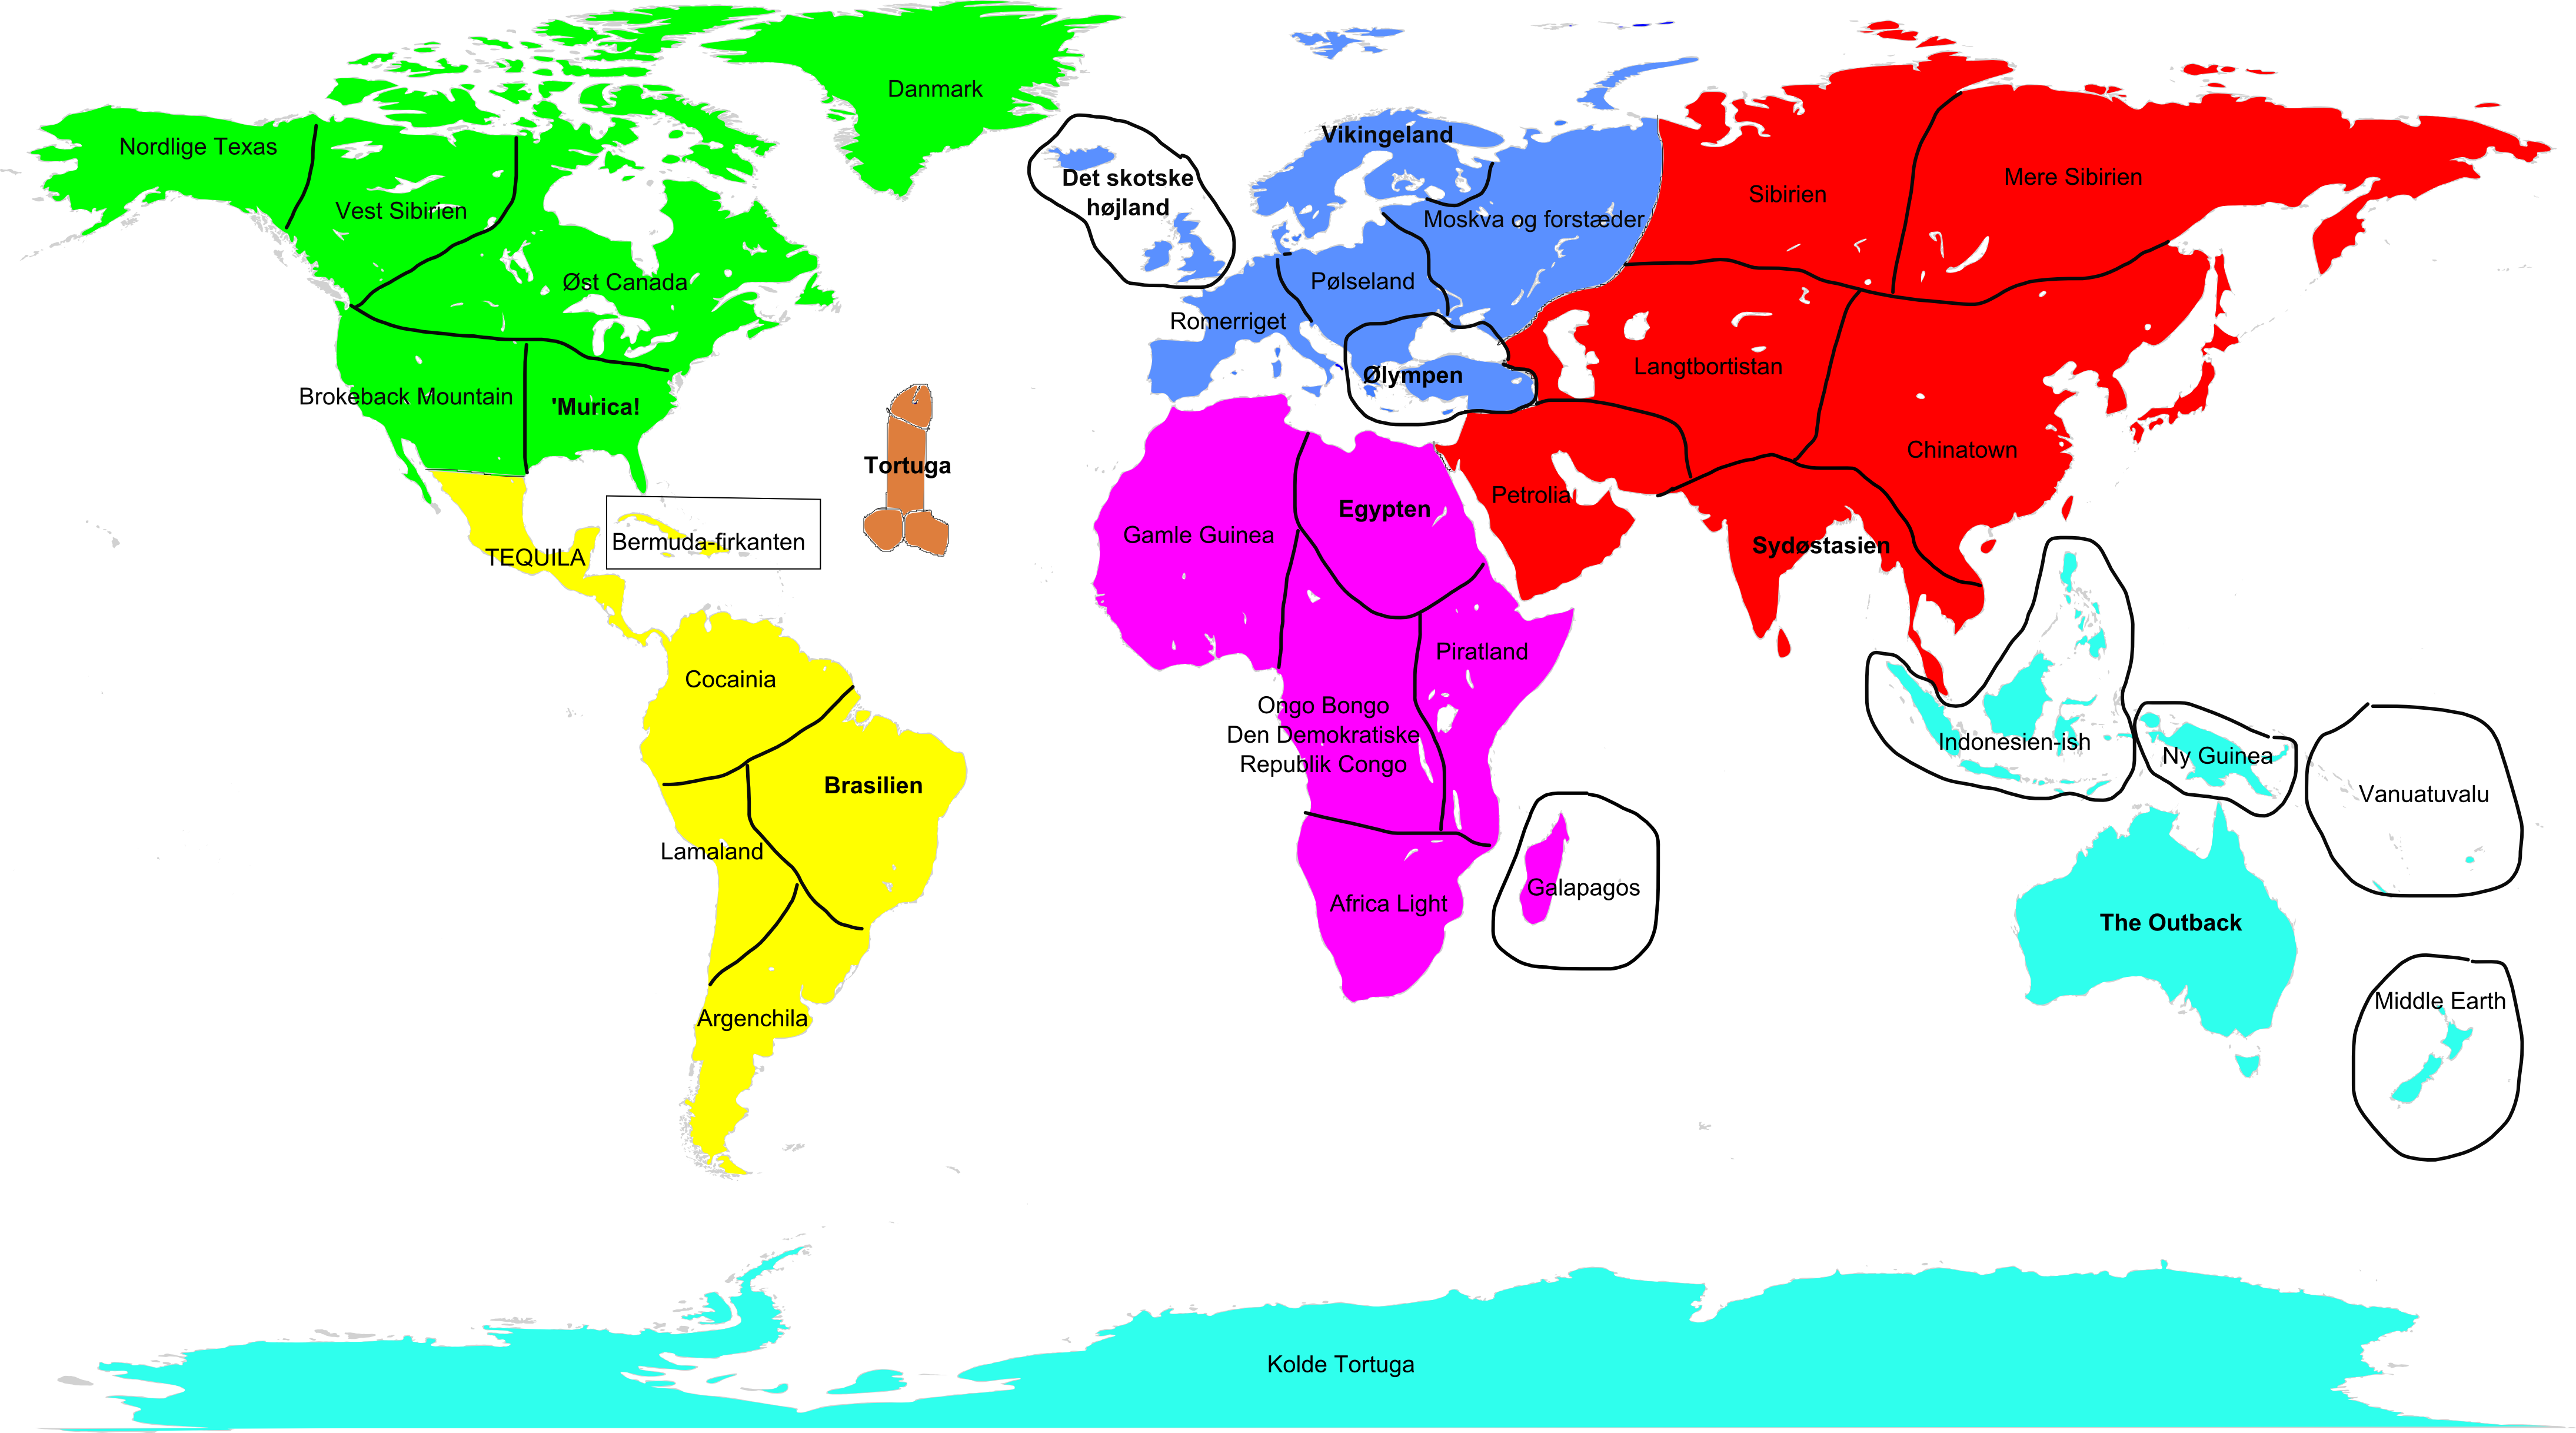
\includegraphics[width=\textwidth]{fig/Verdenskort.png}
\caption{RISK brættet}
\label{fig:RISK}
\end{figure}
$$$$ % "snyde" linjeskift så "Køkken" ryger ned på ny side
\input{tex/div/07-Køkken.tex}
\section{Kompetencelisten}

Hvem kan finde ud af noget, og hvem kan ikke? \Hashtag{RetarderedeVektorer}

\begin{table}[H]
\begin{tabu}{l *{8}{|c}}
\specialrule{1pt}{0pt}{2pt} \rowfont{\bfseries}
Hvem kan hvad       & Stive & Hæmor & Mighty & Buddha & Randi & Karla & Clint & Farav \\ \specialrule{1pt}{2pt}{1pt}
Bræk                & Ja    & Ja    & Ja     & Ja     & Ja    & Nej   & Nej   & Ja    \\ \specialrule{.25pt}{1pt}{1pt}
Blod                & Ja    & Nej   & Ja     & Ja     & Ja    & Ja    & Nej   & Ja    \\ \specialrule{.25pt}{1pt}{1pt}
Knogler             & Nej   & Nej   & Måske  & Ja     & Nej   & Måske & Nej   & Ja    \\ \specialrule{.25pt}{1pt}{1pt}
Rolig tale          & Ja    & Ja    & Ja     & Ja     & Ja    & Ja    & Ja    & Ja    \\ \specialrule{.25pt}{1pt}{1pt}
Taler generelt      & Ja    & Ja    & Ja     & Ja     & Ja    & Måske & Ja    & Ja    \\ \specialrule{.25pt}{1pt}{1pt}
Stoffer (påvirkede) & Ja    & Måske & Måske  & Ja     & Måske & Måske & Måske & Nej   \\ \specialrule{.25pt}{1pt}{1pt}
Aggressive russer   & Ja    & Ja    & Ja     & Ja     & Måske & Ja    & Nej   & Ja    \\ \specialrule{.25pt}{1pt}{1pt}
Ældre               & Ja    & Nej   & Nej    & Ja     & Ja    & Ja    & Ja    & Ja    \\ \specialrule{.25pt}{1pt}{1pt}
Partystarter        & Ja    & Ja    & Ja     & Ja     & Måske & Nej   & Ja    & Ja    \\ \specialrule{.25pt}{1pt}{1pt}
Ædrubonding         & Ja    & Måske & Semi   & Ja     & Ja    & Måske & Ja    & Nej   \\ \specialrule{.25pt}{1pt}{1pt}
Minimal søvn        & Ja    & Ja    & Ja     & Ja     & Ja    & Nej   & Måske & Ja    \\ \specialrule{.25pt}{1pt}{1pt}
Førstehjælp         & Ok    & Ok    & Ok     & Ja     & Ok    & Ja    & Nej   & Ja    \\ \specialrule{1pt}{1pt}{0pt}
\end{tabu}
\end{table}
%\section{Visionsoplæg}
\subsection*{Generelt:}
\underline{\textbf{Formål og retningslinjer:}}\\
Hvad er formålet med rusturen?\\
Russerne skal hinanden at kende og skal ud af deres comfort zone. Få skabt et netværk på hele DTU på tværs af retningerne. 

\underline{\textbf{Holdning til rygning?}}\\
Ingen rygning indenfor. Vi sætter en bænk og spande op, alle skodder skal i spande. 10-sekunders reglen tæller også for skodder. Venlig påmindelse til russer der ikke kan finde ud af det. Opfordr russerne til at spørge om det er ok at ryge i grupperne. Hvis der er skodder over det hele strammes reglerne. 

\underline{\textbf{Holdning til alkohol?}}\\
\textbf{Russer:} Ingen medbragt alkohol. Alt skal indleveres, så får de det tilbage bagefter. Vi holder øje med hvor meget de drikker og kan give for fulde russer vand fra køkkenet. Det er primært ædru-ansvarlige der vurderer om folk er for fulde. Hvis der er nogen der bliver for fuld og til grin, er det en god ide at gribe ind og evt. snakke med de ``højtråbende'' russer.\\
\textbf{Vektor:} Vi har en flaske shots på vektorværelset som man må drikke af hvis man trænger til at få festen startet og ikke kan overskue øl. Man bliver ikke på værelset og safter sig ned, men tager et shot og går ud igen. Vi kan tage et shot til kaosmøderne.\\
Køkkenhold: Har relativt frie tøjler, så længe de kan administrere det og lave god mad til tiden og kan deltage i de aktiviteter, de skal med til. Tager en romtønde med samt fernet. Russerne får klapper for øjnene og en sjat rom til opvasken. Skal en rus have et shot må man gerne lige advare køkkenet på forhånd.

\underline{\textbf{Hash og euforiserende stoffer:}}\\
Nul tolerance. Vi giver dem chancen for at indlevere eventuelt medbragte sager i starten, hvorefter det skylles ud i toilettet med det samme. Dagsansvarlig kigger på mens russen skyller det ud. Hvis vi kan lugte noget, fortælles det til næste samling at det er hjemsendelsesgrund hvis man fanges i at ryge. Hvis stoffer bliver et omfattende problem på turen skal der ringes til Inge, og alle sendes hjem. Er der tale om hårde stoffer (andet end hash), indkaldes der til hastekaosmøde (prik på skulderen) og der ringes til politiet, og de to ædru og russen møder politiet ude ved vejen, så hele rusturen ikke opdager så meget.

\underline{\textbf{Nøgenhed:}}\\
Vi opfordrer ikke til nøgenhed og må ikke selv være nøgne. Smider russerne tøjet bedes de pænt men bestemt om at tage tøj på igen. Gælder også for mankinis. 

\underline{\textbf{Må våben medbringes? Hvad gøres der?}}\\
Nej. Der ringes til politiet. Vi gør opmærksom på det i invitationen. 

\underline{\textbf{Udflugter fra hytten?}}\\
\textbf{Med vektor:} Hvis nogen har lyst vil vektorer gerne løbe en tur om morgenen. Har man overskud kan man gå en tur med nogen.\\ 
\textbf{Uden vektor:} Hvis man gerne vil have en løbetur alene skal man være ædru, og dagsansvarlig kontaktes. Man skal have telefon med. Grunden må ikke forlades fuld uden vektor.

\underline{\textbf{Mobiltelefoner?}}\\
\textbf{Vektorer:} Har for så vidt muligt mobil på sig. Begge ædruveste har altid en opladt telefon på sig. Sørg for at den er ladet op. KABS har mobil på sig hele tiden. Nul sociale medier på turen. Skal man tjekke facebook kan man gøre det inden man går i seng. Slå app-notifikationer fra, så man ikke kommer til at kigge på telefonen hele tiden. Højdere er smart. Vi skaffer en ædrutelefon, som folk kan ringe til og dagsansvarlig har på sig.\\
\textbf{Russer:} Vi opfordrer alle russer til at lade mobilen ligge i tasken, da de ikke er på rustur for at skrive med vennerne. Opkald er ok i nødstilfælde.

\underline{\textbf{Kamera?}}\\
Vi tager et kamera med på turen, russer må gerne tage billeder. Vi laver censur på billederne, der lægges op i den lukkede gruppe på facebook. Vi holder øje med om russerne er for fulde til at håndtere det. Kørselsansvarlig har kameraet.

\underline{\textbf{Håndtering af naboer?}}\\
En vektor tager rundt med telefonnummeret på ædrutelefonen, som de kan ringe til hvis der bliver problemer. 

\underline{\textbf{Håndtering af hyttefar?}}\\
Hyttefar likes, vi gør som han siger. Det er ædruansvarlig der snakker med hyttefar.\\
\textbf{Skader på hytten:} Tag billeder af skader ved ankomst og meld det til hyttefar med det samme. Det samme gælder mangler.\\
\textbf{Uheld:} Der ringes til hyttefar hvis det er seriøst. Russer opfordres til at sige det med det samme, hvis der sker noget. Det hele noteres.\\
\textbf{Hærværk:} Russen betaler selv, og hvis det er seriøst kan der tages stilling til om der skal være yderligere konsekvenser til et kaosmøde.

\subsection*{Russer:}
\underline{\textbf{Gruppepres/indpakning af russer i vat?}}\\
Vi griber ind med liking og andre aktiviteter hvis nogen udsættes for gruppepres. Det er også voksne mennesker, som selv må sige fra nogle gange, så vi skal ikke pakke dem ind i vat. Vi må godt presse dem ud af deres comfort zone, hvis de eksempelvis helst ikke vil være med i en leg. 

\underline{\textbf{Hvad gør vi ved en vektorlegende rus?}}\\
Hvis det ikke bliver for meget må de gerne hjælpe til. Vi bestemmer stadig hvordan tingene forløber. 

\underline{\textbf{Uudholdelige russer?}}\\
En vektor der hverken har vest eller er retningsvektor er bad guy og fortæller stille og roligt russen, at han gør noget som mange synes er irriterende, og at han nok skal stoppe med det. Dette tages først op til et kaosmøde, så alle ved hvad der sker. Virker det ikke, er oversavning altid en mulighed. 

\underline{\textbf{Opmærksomhedskrævende rus?}}\\
Samme situation som ovenfor. Pas på med at save personen over, da det kan eskalere situationen.

\underline{\textbf{Rus, der lægger an på vektor}}\\
Hvis en vektor ser det, gør man den pågældende vektor opmærksom på problemet. Er det et tilbagevendende problem kan man trække russen til side og forklare reglerne for samkvem i studiestarten. Er man i knibe, kan man råbe ananas. 

\underline{\textbf{Russer, der er sammen internt}}\\
Ja tak! Så længe det ikke bliver påtrængende over for de andre. Folk må gerne knalde på værelserne, men ikke andre steder. Det giver badges. Hvis russen beder om ikke at få det offentliggjort til morgenrejsning er dette ok. 

\underline{\textbf{Udlevering af medicin til russer?}}\\
Hvis folk virkelig har brug for en panodil, kan dagsansvarlig udlevere. Man skal holde øje med at folk ikke får for mange. 

\underline{\textbf{En rus med egen bil på turen?}}\\
Inddrager nøglerne indtil turen er slut. Hvis personen mangler noget, kan kørselsansvarlig køre efter det, og det skal aftales på forhånd hvis personen skal køre. Nul tolerance hvis han har drukket. 

\underline{\textbf{Aktivering af stille russer}}\\
Prøv at komme ned på deres niveau, sid og snak med dem og forsøg at få dem med i et spil. Måske ikke et drukspil, men bare en gang Bezzerwizzer eller 500. Prøv at få flere med i spillet, så russen bliver inddraget i en gruppe.

\underline{\textbf{Rus der gerne vil hjem:}}\\
Retningsvektor og evt. tværvektor snakker med russen for at høre om problemet og forsøger at like og overtale russen til at blive. Er det helt skidt tages det op til et haste-kaosmøde. Skal personen hjem, køres russen til nærmeste station, såfremt det er forsvarligt (og russen ikke dør). 

\underline{\textbf{Voldelige russer?}}\\
Dagsansvarlig kontaktes. Der skal mindst to vektorer med. Det kan være farligt at frembruse for offensivt, ofte er det bedre at det er piger der stopper en slåskamp. Tag fat i den ene rus og snak med ham inden det eskalerer og lad situationen køle af. Lad være med at tage side. Få de andre russer væk hvis der opstår en situation. Hvis det går helt galt kan politiet kontaktes.

\underline{\textbf{Kampdrikkende russer:}}\\
Prøv at fortælle dem at der er aktiviteter i løbet af dagen og det vil være smart at holde lidt igen indtil aftensmaden. Fortæl at det er sjovest at være i stand til at deltage i alle aktiviteter. Retningsvektoren kontaktes, så han/hun kan snakke med russen. Er der en der er meget ramt om morgenen skal de med op til morgenrejsning, men de kan få lov til at få en lur hvis de virkelig trænger. 

\underline{\textbf{Klæbende rus:}}\\
Prøv at få involveret russen i aktiviteter med andre russer ala den stille rus. Man kan godt opfordre dem til at snakke med de andre russer. Alternativt kan man smide russen af på en anden vektor.

\underline{\textbf{Opsyngning:}}\\
Man synger ikke enkelte personer op. Hold det på et minimum til morgenmad (og frokost), og lad være med at få det til at eskalere under aftensmaden. Ædruansvarlig kan gå rundt til de andre vektorer og bede om ro hvis det stikker for meget af. Man må ikke bare overdøve et hold med ``man drikker hvis man ikke kan synge''.
\subsection*{Interne problemer:}
\underline{\textbf{Vektor er sammen med rus:}}\\
Vi hiver vektoren og russen til side og forklarer, at det var en fejl men det ikke var russens skyld. Vektoren er ædru resten af turen, og KABS finder ud af om der skal ske yderligere konsekvenser. Der uddeles ikke scorebadges.

\underline{\textbf{Fuld under/før ædruvagt:}}\\
Ædru resten af turen. Man får en ny vagt. Den mindst fulde bliver hurtigt ædru og overtager. Den resterende ædruvest får begge veste. 

\underline{\textbf{Uenighed:}}\\
Dagsansvarlig har sidste ord. Flyt diskussionen ind på vektorværelset så vi ikke står og diskuterer foran russerne. Lad være med at rette på folk foran russerne. Hvis man bliver uvenner snakker man med KABS om problemet. Det er en god ide lige at få sovet på det og så få snakket om det dagen efter. 

\underline{\textbf{Dovenskab:}}\\
Find dagsansvarlig eller KABS. Der skal likes. Hvis man har brug for en powernap spørger man lige dagsansvarligt.  

\underline{\textbf{Andres ansvarsposter:}}\\
Vi stoler på at de ansvarlige har styr på deres ting, og at man spørger om hjælp hvis man har brug for det. 

\subsection*{Interne forventninger og aftaler}
\underline{\textbf{Forventninger til madholdet?}}\\
God mad til tiden og rom og kaffe og fernet tak. Og kolde øl hvis der er plads. Kan hjælpe til med løb. Tager gerne imod russer der har brug for en pause, hvis de bliver advaret på forhånd. Tidsændringer meldes til køkkenet i god tid. Dagsansvarlig holder styr på det. Der kommer en pirat med til alle kaosmøder. Forsinkelser i køkkenet meldes også i god tid.  I køkkenet bestemmer piraterne. Vil gerne have drejebog.

\underline{\textbf{Hvad forventes der af ædruvagter?}}\\
Begge veste skal kunne udgå fra løb uden problemer, hvis der skulle opstå noget.\\
\textbf{Dagsansvarlig:} Helst være ædru tak. Har de endelige beslutninger. Holder styr på at tidsplanen overholdes i løbet af dagen. Har kontakten til køkkenet. Indkalder til kaosmøder og har styr på dagsordenen. Holder orden til måltiderne og giver beskeder eller får en med en god stemme til det. Har fuldstændig styr på hvad der skal ske i løbet af dagen. Har kontakt til den anden vest. Husk at spørge om hjælp og uddeleger.\\
\textbf{Kørselsansvarlig:} Ædru, kan køre bil. Skal være frisk nok til at køre bil, så man må gerne tage en lur. Giver besked til dagsansvarlig hvis man tager en lur. Bunder når vesten lægges. Hjælper dagsansvarlig hvor der er brug for det. Tager billeder!\\
\textbf{Overdragelse af veste:} Bunder en øl/cocio, men styrer alligevel sin brandert. 

\underline{\textbf{Hvad er jeres ansvar og forventninger som vektorer til hinanden:}}\\
Man saver sig ikke ned så man ikke kan tage ansvar. Ølbowling inden ansvar er en dårlig ide. Der er hovedansvarlige for alle ting, men alle skal vide hvad der sker på turen. Vi bakker hinanden op og hjælper hvis vi ser der er brug for det. Man er stadig vektor selvom man ikke har vest på.  

\underline{\textbf{Forholdet mellem sjov og seriøse ting:}}\\
Der kommer til at være lidt af hvert. 

\underline{\textbf{Førstehjælpskassens placering:}}\\
I køkkenet.

\underline{\textbf{Forholdet mellem tid i retnings og tværholdet:}}\\
Primært tværholdet, da man er sammen med retningen resten af året. Ingeniøropgaven bliver i retning, og måske et løb. 

\addcontentsline{toc}{subsection}{Kompetencelisten}

\underline{\textbf{Hvem er gode til hvilke situationer:}} Bræk, blod, rolig tale, førstehjælp osv.?\\

\begin{table}[H]
\begin{tabu}{l *{8}{|c}}
\specialrule{1pt}{0pt}{2pt} \rowfont{\bfseries}
Hvem kan hvad       & Stive & Hæmor & Mighty & Buddha & Randi & Karla & Clint & Farav \\ \specialrule{1pt}{2pt}{1pt}
Bræk                & Ja    & Ja    & Ja     & Ja     & Ja    & Nej   & Nej   & Ja    \\ \specialrule{.25pt}{1pt}{1pt}
Blod                & Ja    & Nej   & Ja     & Ja     & Ja    & Ja    & Nej   & Ja    \\ \specialrule{.25pt}{1pt}{1pt}
Knogler             & Nej   & Nej   & Måske  & Ja     & Nej   & Måske & Nej   & Ja    \\ \specialrule{.25pt}{1pt}{1pt}
Rolig tale          & Ja    & Ja    & Ja     & Ja     & Ja    & Ja    & Ja    & Ja    \\ \specialrule{.25pt}{1pt}{1pt}
Taler generelt      & Ja    & Ja    & Ja     & Ja     & Ja    & Måske & Ja    & Ja    \\ \specialrule{.25pt}{1pt}{1pt}
Stoffer (påvirkede) & Ja    & Måske & Måske  & Ja     & Måske & Måske & Måske & Nej   \\ \specialrule{.25pt}{1pt}{1pt}
Aggressive russer   & Ja    & Ja    & Ja     & Ja     & Måske & Ja    & Nej   & Ja    \\ \specialrule{.25pt}{1pt}{1pt}
Ældre               & Ja    & Nej   & Nej    & Ja     & Ja    & Ja    & Ja    & Ja    \\ \specialrule{.25pt}{1pt}{1pt}
Partystarter        & Ja    & Ja    & Ja     & Ja     & Måske & Nej   & Ja    & Ja    \\ \specialrule{.25pt}{1pt}{1pt}
Ædrubonding         & Ja    & Måske & Semi   & Ja     & Ja    & Måske & Ja    & Nej   \\ \specialrule{.25pt}{1pt}{1pt}
Minimal søvn        & Ja    & Ja    & Ja     & Ja     & Ja    & Nej   & Måske & Ja    \\ \specialrule{.25pt}{1pt}{1pt}
Førstehjælp         & Ok    & Ok    & Ok     & Ja     & Ok    & Ja    & Nej   & Ja    \\ \specialrule{1pt}{1pt}{0pt}
\end{tabu}
\end{table}

\underline{\textbf{Rus lægger an på vektor - hvordan stoppes det?}} (sang, bestemt sætning e.l.?)\\
Kald på en vektor i nærheden. Hvis man ser det, kan man hente vektoren udenfor. Ananas og kigge på stjerner. 

\underline{\textbf{Hvor mange vektorer er vågne pr rus? Hvem må lukke festen?}}
Er det ok at 2 vektorer/KABS er vågne og holder styr på festen, hvis 30 russer er oppe?\\
Vektorerne lukker og slukker, selvom der er 10-15 stykker der stadig gerne vil feste. Sig at vi også har et program for morgendagen. Musikcomputeren kan bare slukkes. Der skal være mindst to vektorer vågne uanset antallet af russer. Dagsansvarlig skal godkende at vektorerne går i seng. Medmindre dagsansvarlig sover, i så fald vendes det bare blandt de resterende vektorer. Dagsansvarlig giver ``ansvaret'' til den mindst fulde vektor. Det kan også aftales til kaosmøder. 

\underline{\textbf{Hvornår sendes folk i seng?}}\\
Kl. 4 senest. 

\underline{\textbf{Søvn - hvor og hvor meget må vi sove?}}\\
Dagsansvarlig skal sørge for at have sovet så meget ud som muligt inden sin vagt. Ellers spørger man dagsansvarlig om man må tage en powernap i løbet af dagen. 

\underline{\textbf{Kaosmøder - hvordan og hvor ofte?}}\\
Morgenmøder er en god ide. Vi ser på den overordnede plan for at vurdere om vi skal have et møde senere på dagen også. Dagsansvarlig gennemgår hvad der skal ske i løbet af dagen, og de ting der er sket tages op. Der findes ud af hvem der skal have hvilke badges og hvad der skal læses op af sladderkassen. 

\subsection*{Generelle regler:}

\underline{\textbf{Alkoholpolitik - vektorer}}\\
Når vagten indtræder, skal den ansvarlige være 100 \% ædru. Man skal senest
stoppe med at drikke, 16 timer får vagten indtræder. Alle ansvarlige skal
stoppe med at drikke torsdag midnat.

\underline{\textbf{Autoritet}}\\
Tilegnede refleksveste skal bæres under hele vagten. Ædruvagt har ALTID sin
mobil på sig.

\underline{\textbf{Overlevering}}\\
Før en vagt afsluttes, skal en overlevering til de efterfølgende kørsels- og
dagsansvarlige ske. Sker der noget under overleveringen, som kræver kørsel,
kører den daværende kørselsansvarlige.

\underline{\textbf{Drejebogen}}
Hvis man mister sin drejebog og en rus finder den, skylder man en øl til
russen. Hvis man mister drejebogen helt, og den ikke bliver fundet på turen
skylder man en kasse til vektorerne. 


%\section{Materiale liste}
\subsubsection*{Inkøbsliste}
\begin{itemize}
  \item 2 ruller Gaffatape
  \item 40 træklemmer
  \item 300 stk marie kiks
  \item 16 fyrfadslys
  \item 16 lightere (evt. tændstikker)
  \item 2kg mel
  \item 2kg salt
  \item 1,5L vand
  \item 2-3dL madolie
  \item 100m snor (muresnor)
  \item Elefant-snot
  \item 150 engangskrus (med kant, så de kan holdes med tænderne)
  \item 2 ruller snor
  \item 1 lagen
  \item 2L græsk yoghurt(lav fedtprocent)
  \item 3L boksrødvin
  \item 25 Skeer(store, plastik)
  \item 30 Grønne servietter
  \item 30 Røde servietter
  \item 2-3 cykelslanger
  \item 2-3 bamse-lignende ting
  \item 2 flasker vodka
  \item 1 flaske hyldeblomstsaft
  \item 6L danskvand
  \item 6 lime
  \item Kål
  \item Galliano (store mængder)
  \item Vodka (store mængder)
  \item Kahlúa (store mængder)
\end{itemize}
    
\subsubsection*{Andre Materialer}
\begin{itemize}
  \item presenninger ved regn/dårligt løb
  \item 8 ølkasser/mælkekasser
  \item Laminerede "kort" (printes på forskellige farver papir, så der kan kendes forskel på nemme og svære)
  \item RISK-plade (hjemmeprintet og lamineret A2)
  \item Lande-labels (2 sæt, lamineret)
  \item 2 baljer
  \item 3 Sakse
  \item 8 Kuglepen
  \item 8 Stopur (vores mobiler)
  \item Klodsmajor(højst sandsynlig fra badekar)
  \item Spyd(gren)
  \item Målebånd
  \item Papir
  \item Vitawrap
  \item 24 dåser fra bussen
  \item slangebøsse (laves af gren og elastik)
  \item Skilte med meter
  \item 2 hulahopringe
  \item Ipod med sange
  \item Høretelefoner
  \item Bat
  \item Krokketkugle
  \item Avis
  \item Sav/hammer/værktøj
  \item Dæk \Stive
\end{itemize}


Fra Visions oplæg:
\begin{itemize}
  \item Rygespande
  \item 3 flasker shots til vektorværelset
  \item SIM-kort / taletidskort
  \item Panodil
  \item 3 walkies
\end{itemize}

\section*{Almindelig førstehjælp på Rustur:} Her er en liste over ting I kan komme ud for på rusturene:

\begin{itemize}
\item \textit{\textbf{Fremmedlegemer i luftvejende}}: Ved delvist blokeret (patienten kan godt sige noget) opfordres der til hoste og evt. slag med flad hånd mellem skuldrebladene, samtidig med hoste. Ved total blokering anbefales det, at der veksles mellem at give 5 slag mellem skuldrebladene og 5 hårde stød i bughulen op mod mellem gulvet, Heimlich (armene rundt om patient der bøjer sig forover).\\
\item \textbf{\textit{Hjernerystelse:}} Kommer til udtryk ved en eller flere af følgende symptomer: Hovedpine, Kvalme, Opkast, Svimmelhed, Synsforstyrrelser, Træthed og tap af korttidshukommelse. Førstehjælpen er: Læg personen for at slappe af/sove og hold tæt observation i mindst 24 timer, f.eks. ved at vække personen en gang i timen. Dette er for at sikre, at tilstanden ikke forværres. Bliver personen tiltagende dårlig, skal der søges skadestue eller læge hurtigst muligt. \\
\item \textbf{\textit{Forbrænding}}: Mindre forbrændinger skal straks køles ned med, så koldt vand som patienten kan holde ud, indtil det ikke gør ondt længere. Sværere forbrændinger (2. grads kan ses ved at der er vabler/sår og 3. grads vil huden være lederagtig og blødende) skylles med tempereret vand (ca. 18-19 grader), der alarmeres og skylning fortsætter under transport til videre behandling. \\
\item \textbf{\textit{Hedeslag/solstik}}: Symptomer: hovedpine, svimmelhed og træthed. Huden vil være varm og lyserød. Patienten vil svede og være konfus. Førstehjælpen er at få patienten i skygge og fjern/løsne tøj. Læg koldt omslag ved pande, nakke, håndled, lyske og ankler, giv noget koldt at drikke. \\
\item \textbf{\textit{Knoglebrud}}: Ved ben- eller bækkenbrud tilkald ambulance og støt bruddet i findestillingen. Ved mindre brud kan man køre selv og holde bruddet i ro, evt med trekant tørklæde. \\
\item \textbf{\textit{Forstuvning}}: Opstår ved for stor og forkert belastning af et led, symptomerne kan afhjælpes ved at benytte sig af {\color{red}\textbf{R.I.C.E}}-princippet:
\begin{itemize}
\item[{\color{red}\textbf{R}} =] Rest. Hold det beskadigede område i ro i det første døgn.
\item[{\color{red}\textbf{I}} =] Ice. Afkøl med is(køleposer kan bruges) eller koldt vand. Køl i ca. 30 min. og hold derefter en times pause. Fortsæt dette til hørelsen er aftaget.
\item[{\color{red}\textbf{C}} =] Compression. Sørg for at lægge pres på det beskadigede sted øjeblikkeligt, hold det i ca. 10-20 min og anlæg derefter et støttebind. 
\item[{\color{red}\textbf{E}} =] Elavation. Løft det beskadigede område over hjerte højde. \\
\end{itemize}
\item \textbf{\textit{Snitsår}}: Rens med renseservietter og sæt plaster på, brug evt. lille kompresforbinding. Løft for at standse blødning.\\
\item \textbf{\textit{Næseblod}}: Pres 2 fingre på næsen og bøj hovedet let forover. Læg evt en kold klud eller is over næsen, for at få blodkar til at trække sig sammen. Hvis blødningen ikke er stoppet efter en halv time så søg læge eller skadestue. \\
\item \textbf{\textit{Flåt}}: Fjern flåten med flåt-tang. Mas aldrig på kroppen af flåten. Kan den ikke fjernes, søg læge. \\
\item \textbf{\textit{Bistik}}: Hvis man bliver stukket i  mund eller hals skal der søges læge eller skadestue, er dette langt væk, tilkald ambulance. Normale bistik kan afhjælpes med en sukkerknad, der trækker giften ud, husk at se om brodden er kommet ud. \\
\item \textbf{\textit{Astma}}: Ved anfald, støt personen i at sidde eller stå. De skal ikke ligge ned, da dette kan forværre åndenøden. Armene over hovedet kan også hjælpe. Sørg for frisk luft og giv psykisk førstehjælp. Evt. hjælp med personens egen medicin eller astmaspray. \\
\item \textbf{\textit{Diabetes}}: Skyldes nedsat eller ingen produktion af hormonet insulin, der transporterer sukker fra blod ind i cellerne. Anfald kan skyldes lavt eller højt blodsukker. Ved lavt blodsukker gives noget sødt at spise eller drikke. Ellers trinvis førstehjælp. Er man i tvivl om det er højt eller lavt blodsukker så giv noget sødt alligevel, da det ikke gør den store forskel, hvis blodsukkeret allerede er for højt. Man må ikke selv give insulin til sukkersygepatienter. Hvis de er ved bevidsthed kan man hjælpe, de har som regel selv helt styr på det. \\
\item \textbf{\textit{Epilepsi}}: Få personen til at ligge ned og løsne stramt tøj om halsen. Beskyt hovedet mod stød, når krampen ophører lægges personen i stabilt sideleje for at skabe frie luftveje. De vil oftest være meget trætte. Forsøg ikke at stikke noget mellem tænderne, men forhold dig i ro.
\end{itemize}
\section{Kørselsvejledninger}
\subsection{DTU til Center Sjælland}
Anker Engelunds Vej 1, 2800 Kongens Lyngby til Køgevej 55, 4690 Haslev.
\begin{itemize}
\item Tag mod øst ad Anker Engelunds Vej mod Kollegiebakken
\item Drej til højre, og følg Lundtoftegårdsvej
\item Drej til venstre, og følg Klampenborgvej
\item Hold til højre, og flet sammen med Rute 19/E47/E55 mod Rødby/København
\item Hold til højre for at fortsætte mod frakørsel Avedøre
\item Ved udfletningsanlægget Avedøre skal du holde mod højre og følge skiltene for E20v/E47/E55 mod Odense/Rødby/Gedser
\item Flet sammen med E20/E47/E55
\item Hold til højre, og følg skiltene mod Rødby/Gedser
\item Tag frakørsel 35-Haslev mod 151/Dalby
\item Drej til højre, og følg Køgevej (skilte til Haslev) Destinationen vil ligge på højre side.
\end{itemize}

\subsection{Center Sjælland til Køge Skadestue}
Køgevej 55, 4690 Haslev til Lykkebækvej 1, 4600 Køge
\begin{itemize}
\item Tag mod nordøst ad Køgevej mod Charlottedalsvej
\item Drej til venstre, og flet sammen med E47/E55 mod København
\item Flet sammen med E20/E47/E55
\item Tag frakørsel 32-Køge mod Ølby/Havn/Færge
\item Drej til højre, og følg Lyngvej
\item Drej til højre ad den 1. vej, og fortsæt ad Stensbjergvej
\item Drej til højre, og følg Lykkebækvej
\item Drej til venstre ad den 1. vej for at blive på Lykkebækvej
\item Kør ind i rundkørslen, destinationen vil ligge på højre side.
\end{itemize}

\subsection{Center Sjælland til Netto}
Køgevej 55, 4690 Haslev til Stationspladsen 2, 4690 Haslev
\begin{itemize}
\item Tag mod sydvest ad Køgevej mod Freerslev Bygade
\item Drej til højre, og følg Københavnsvej
\item Fortsæt ad Gamle By
\item Lidt til højre, og følg Kirkepladsen, kør gennem 1 rundkørsel
\item Forsæt ad Præstevænget
\item Forsæt lige ud ad Tingvej
\item Drej til højre, og følg Stationsvej
\item Fortsæt ad stationspladsen, destinationen vil ligge på højre side.
\end{itemize}

\begin{figure}[H]
\begin{center}
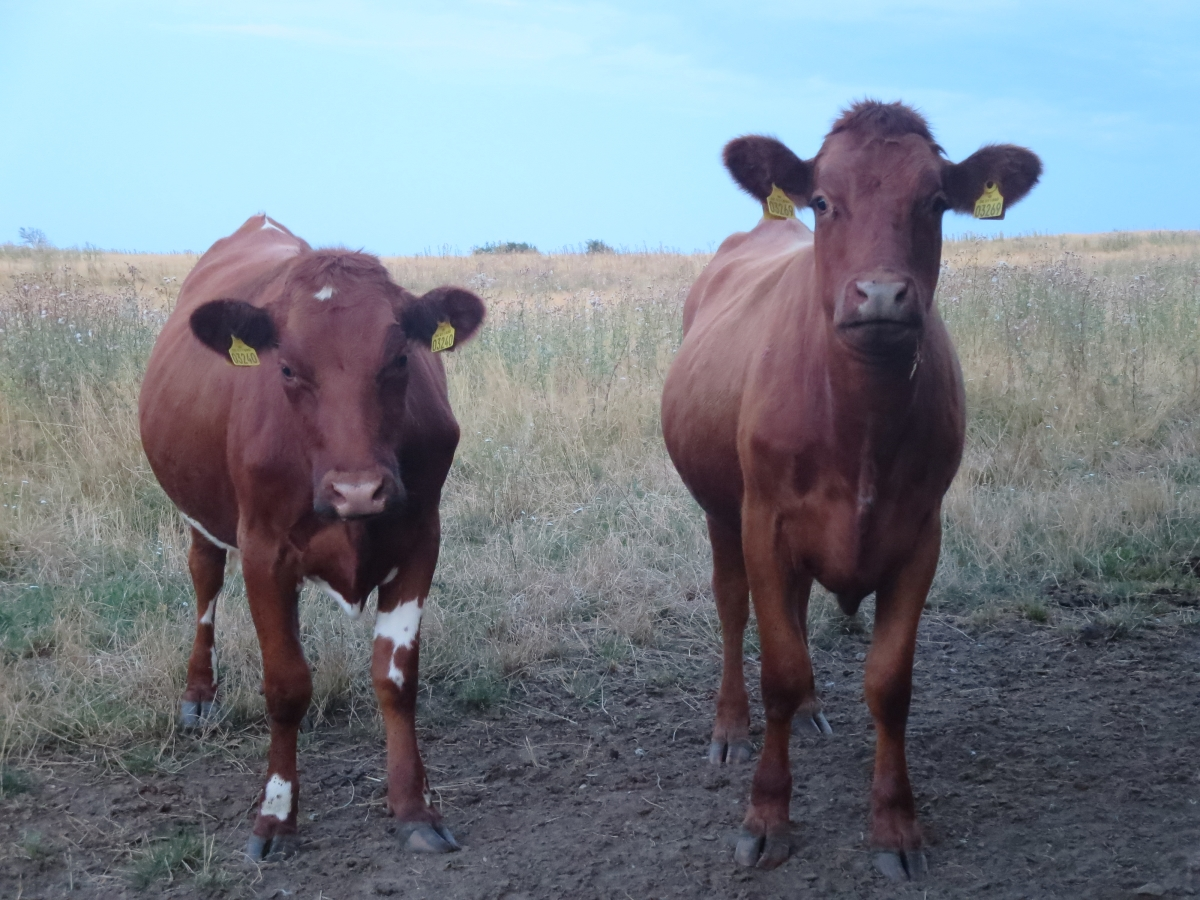
\includegraphics[width=\textwidth]{fig/Ko.JPG}
\end{center}
\end{figure}

\pagebreak % skal være bagerst. På en side for sig selv.

\section{Praktisk}
\vspace{-0.3cm}
\subsection{Telefonnumre}
\vspace{-0.5cm}
\begin{table}[H]
\centering
\begin{tabu}{L{3cm} L{5cm} r}\specialrule{1pt}{0pt}{2pt}
\rowfont{\bfseries}
Hvad & Hvem & \multicolumn{1}{l}{Tlf} \\ \specialrule{1pt}{2pt}{2pt}
Dagsansvarlig           & (Elizabeths telefon)              & \textbf{61 79 XX XX} \\ \specialrule{.25pt}{1pt}{1pt}
KABS                    & \Farav                            & 61 46 XX XX \\ \specialrule{.25pt}{1pt}{1pt}
\multirow{7}{*}{Vektor} & \Clint                            & 28 77 XX XX \\
						& \Randildo                         & 23 44 XX XX \\
						& \Karla                            & 61 18 XX XX \\
						& \Stive                            & 40 29 XX XX \\
						& \Buddha                           & 31 49 XX XX \\
						& \Mighty                           & 53 57 XX XX \\
						& \Hemorides                        & 24 29 XX XX \\ \specialrule{.25pt}{1pt}{1pt}
\multirow{3}{*}{Bumz}   & \Hyttebums{Captain Jack Swallows} & 28 90 XX XX \\
					    & \Hyttebums{Elizabeth Porn}        & 61 79 XX XX \\
					    & \Hyttebums{William Turn-On}       & 30 35 XX XX \\ \specialrule{.25pt}{1pt}{1pt}
PF                      & Inge                              & 77 42 XX XX \\ \specialrule{.25pt}{1pt}{1pt}
Hyttefar                & Svend Ole Svendsen                & 52 88 XX XX \\ \specialrule{.25pt}{1pt}{1pt}
Lægevagt                & Åben hverdage kl. 16:00-08:00     & 70 15 XX XX \\
Skadestue               &                                   & 56 63 15 XX \\ \specialrule{.25pt}{1pt}{1pt}
\multirow{2}{*}{Politi} & Midt \& Vest-                     & 114         \\
                        & Sjælland                          & 46 35 14 48 \\ \specialrule{1pt}{2pt}{0pt}
\end{tabu}
\end{table}
\vspace{-0.5cm}


\subsection{Adresser}
\vspace{-0.5cm}
\begin{table}[H]
\centering
\begin{tabu}{lll}\specialrule{1pt}{0pt}{2pt}
\rowfont{\bfseries}
Hvad & Adresse & Tlf \\ \specialrule{1pt}{2pt}{1pt}
Center Sjælland & \doublecell{Køgevej 55\\4690 Haslev} & \\ \specialrule{.25pt}{1pt}{1pt}
Skovfoged: Jesper Jørgensen & \doublecell{Østerskovvej 19\\4682 Tureby} & \\ \specialrule{.25pt}{1pt}{1pt}
\doublecell{Skadestue/Akutafdeling\\Køge sygehus} & \doublecell{Lykkebækvej 1 – indgang 11/13\\4600 Køge} & \\ \specialrule{.25pt}{1pt}{1pt}
Køge Apotek & \doublecell{Brogade 1\\4600 Køge} & 56 65 01 21\\ \specialrule{.25pt}{1pt}{1pt}
Netto & \doublecell{Stationspladsen 2\\4690 Haslev} & \\ \specialrule{.25pt}{1pt}{1pt}
Helsingør Turisttrafik & \doublecell{Fabriksvej 1\\3000 Helsingør} & 49 22 33 33\\ \specialrule{.25pt}{1pt}{1pt}
\doublecell{Giftlinjen\\Bispebjerg Hospital} & \doublecell{Bispebjerg Bakke 23\\2400 København NV} & 82 12 12 12\\ \specialrule{1pt}{1pt}{0pt}
\end{tabu}
\end{table}
\vspace{-0.5cm}

Du skal altid ringe først til Region Sjællands akuttelefon på 70 15 07 08, hvis du kommer til skade. I telefonen guider sygeplejersker dig videre til den rigtige og hurtigste hjælp. Du kan ikke møde op uden en aftale! Ring ikke til Akuttelefonen i tilfælde af livstruende situationer og ulykker. Ring i stedet 112. % skal være til sidst (eller helt i starten)

\end{document}